\documentclass[titlepage]{article}

\usepackage{fancyhdr}
\usepackage{hyperref}
\usepackage{titlesec}
\usepackage{graphicx}
\usepackage{tikz}
\usepackage{listings}
\usepackage{xcolor}
\usepackage{float}
\usepackage[font=itshape]{quoting}
\definecolor{codegreen}{rgb}{0,0.6,0}
\definecolor{codegray}{rgb}{0.5,0.5,0.5}
\definecolor{codepurple}{rgb}{0.58,0,0.82}
\definecolor{backcolour}{rgb}{0.95,0.95,0.92}
\definecolor{lightgray}{rgb}{0.95, 0.95, 0.95}
\definecolor{darkgray}{rgb}{0.4, 0.4, 0.4}
\definecolor{purple}{rgb}{0.65, 0.12, 0.82}
\definecolor{ocherCode}{rgb}{1, 0.5, 0} % #FF7F00 -> rgb(239, 169, 0)
\definecolor{blueCode}{rgb}{0, 0, 0.93} % #0000EE -> rgb(0, 0, 238)
\definecolor{greenCode}{rgb}{0, 0.6, 0} % #009900 -> rgb(0, 153, 0) 

\lstdefinestyle{mystyle}{
    backgroundcolor=\color{backcolour},   
    commentstyle=\color{codegreen},
    keywordstyle=\color{magenta},
    numberstyle=\tiny\color{codegray},
    stringstyle=\color{codepurple},
    basicstyle=\ttfamily\footnotesize,
    breakatwhitespace=false,         
    breaklines=true,                 
    captionpos=b,                    
    keepspaces=true,                 
    numbers=left,                    
    numbersep=5pt,                  
    showspaces=false,                
    showstringspaces=false,
    showtabs=false,                  
    tabsize=2
}

\lstdefinelanguage{JavaScript}{
  keywords={typeof, new, true, false, catch, function, return, null, catch, switch, var, if, in, while, do, else, case, break},
  keywordstyle=\color{blue}\bfseries,
  ndkeywords={class, export, boolean, throw, implements, this, extends, import},
  ndkeywordstyle=\color{orange}\bfseries,
  identifierstyle=\color{black},
  literate={
        {\ \ }{{\ }}1
    },
  sensitive=false,
  comment=[l]{//},
  morecomment=[s]{/*}{*/},
  commentstyle=\color{purple}\ttfamily,
  stringstyle=\color{red}\ttfamily,
  morestring=[b]',
  morestring=[b]",
}

\lstdefinelanguage{CSS}{
      keywords={accelerator,azimuth,background,background-attachment,
            background-color,background-image,background-position,
            background-position-x,background-position-y,background-repeat,
            behavior,border,border-bottom,border-bottom-color,
            border-bottom-style,border-bottom-width,border-collapse,
            border-color,border-left,border-left-color,border-left-style,
            border-left-width,border-right,border-right-color,
            border-right-style,border-right-width,border-spacing,
            border-style,border-top,border-top-color,border-top-style,
            border-top-width,border-width,bottom,caption-side,clear,
            clip,color,content,counter-increment,counter-reset,cue,
            cue-after,cue-before,cursor,direction,display,elevation,
            empty-cells,filter,float,font,font-family,font-size,
            font-size-adjust,font-stretch,font-style,font-variant,
            font-weight,height,ime-mode,include-source,
            layer-background-color,layer-background-image,layout-flow,
            layout-grid,layout-grid-char,layout-grid-char-spacing,
            layout-grid-line,layout-grid-mode,layout-grid-type,left,
            letter-spacing,line-break,line-height,list-style,
            list-style-image,list-style-position,list-style-type,margin,
            margin-bottom,margin-left,margin-right,margin-top,
            marker-offset,marks,max-height,max-width,min-height,
            min-width,-moz-binding,-moz-border-radius,
            -moz-border-radius-topleft,-moz-border-radius-topright,
            -moz-border-radius-bottomright,-moz-border-radius-bottomleft,
            -moz-border-top-colors,-moz-border-right-colors,
            -moz-border-bottom-colors,-moz-border-left-colors,-moz-opacity,
            -moz-outline,-moz-outline-color,-moz-outline-style,
            -moz-outline-width,-moz-user-focus,-moz-user-input,
            -moz-user-modify,-moz-user-select,orphans,outline,
            outline-color,outline-style,outline-width,overflow,
            overflow-X,overflow-Y,padding,padding-bottom,padding-left,
            padding-right,padding-top,page,page-break-after,
            page-break-before,page-break-inside,pause,pause-after,
            pause-before,pitch,pitch-range,play-during,position,quotes,
            -replace,richness,right,ruby-align,ruby-overhang,
            ruby-position,-set-link-source,size,speak,speak-header,
            speak-numeral,speak-punctuation,speech-rate,stress,
            scrollbar-arrow-color,scrollbar-base-color,
            scrollbar-dark-shadow-color,scrollbar-face-color,
            scrollbar-highlight-color,scrollbar-shadow-color,
            scrollbar-3d-light-color,scrollbar-track-color,table-layout,
            text-align,text-align-last,text-decoration,text-indent,
            text-justify,text-overflow,text-shadow,text-transform,
            text-autospace,text-kashida-space,text-underline-position,top,
            unicode-bidi,-use-link-source,vertical-align,visibility,
            voice-family,volume,white-space,widows,width,word-break,
            word-spacing,word-wrap,writing-mode,z-index,zoom},  
      sensitive=true,
      morecomment=[l]{//},
      morecomment=[s]{/*}{*/},
      morestring=[b]',
      morestring=[b]",
      alsoletter={:},
      alsodigit={-}
    }

\lstset{style=mystyle}

\usetikzlibrary{shapes,arrows}
\newcommand{\comment}[1]{}


\tikzstyle{decision} = [diamond, draw, 
    text width=4.5em, text badly centered, node distance=3cm, inner sep=0pt]
\tikzstyle{line} = [draw, -latex']
\tikzstyle{block} = [rectangle, draw, 
    text width=8em, text centered, rounded corners, minimum height=4em]
\tikzstyle{start} = [rectangle, draw, 
    text width=4.5em, text badly centered, rounded corners, node distance=3cm]
\tikzstyle{io} = [trapezium, trapezium left angle=70, trapezium right angle=110, minimum width=3cm, minimum height=1cm, text centered, draw=black]


\setcounter{secnumdepth}{5}
\setcounter{tocdepth}{4}

\pagestyle{fancy}
\fancyhf{}
\rhead{Path-finding Algorithms and Solving Mazes}
\lhead{Oliver Temple [CN]}
\rfoot{\thepage}
\lfoot{Path-finding Algorithms and Solving Mazes}

\title{Path-finding Algorithms and Solving Mazes}

\author{Oliver Temple}

\begin{document}

\maketitle
\tableofcontents

\section{analysis}
\subsection{Project Description}
Path finding algorithms are essential in many aspects of computer science, from computer games to solving complex real world problems, however they can be complex things to visualize, especially when learning about them for the first time. This project's aim to create a path finding visualization tool that will generate and solve mazes, and to provide a general understanding of the algorithms used. 

There are a number of different algorithms that can be used to solve and generate mazes, and this project will focus on the more common ones like Dijkstra's, Depth First Search, Prims and more. I intend to include algorithms that are different from each other to show the advantages and disadvantages of each.

\subsection{Research}
\subsubsection{Overview}
To complete this project, I will need a strong understanding of maze generation and path finding algorithms, how they work and how to model them, knowledge of react and javascript to create a website for the visualization as well as user opinions on what features are needed.
\subsubsection{Research Log}
I was introduced to path finding algorithms in one of my lessons, where we learned what they were used for and some examples, as well as how they can be modeled. For example, modelling the maze as a graph with weighted nodes of 1 and 0, for the walls and space respectively. The algorithms we looked at were Dijkstra's and A*. We also looked at Prim's algorithm, recursive backtracking, depth fist search and Kruskal's algorithms for maze generation.

\paragraph{Maze Generating Algorithms}
\subparagraph*{Prims}
In class, we were taught about Prim's algorithm, and how it works. I used the information that our teacher gave us to write my own implementation of Prim's algorithm.
\subparagraph*{Recursive Backtracking}
When researching recursive backtracking I can across a website that said:
\begin{quoting}
    Here's the mile-high view of recursive backtracking:
    \begin{enumerate}
        \item Choose a starting point in the field.
        \item Randomly choose a wall at that point and carve a passage through to the adjacent cell, but only if the adjacent cell has not been visited yet. This becomes the new current cell.
        \item If all adjacent cells have been visited, back up to the last cell that has uncarved walls and repeat.
        \item The algorithm ends when the process has backed all they way up to the starting point. 
    \end{enumerate}
\end{quoting}
\url{https://weblog.jamisbuck.org/2010/12/27/maze-generation-recursive-backtracking}
I used this along with another visualization that I found to write my own recursive backtracking algorithm.

\paragraph{Path Finding Algorithms}
\subparagraph*{Depth First Search}
For the depth first search, I looked \url{https://isaaccomputerscience.org/concepts/dsa_pathfinding_dfs_bfs?examBoard=ocr&stage=a_level}, a resource I often use for studying. I used their easy to understand description to write my own implementation of depth first search. Their website said:
\begin{quoting}
    A depth-first search begins at the start node and then searches as far as possible down a branch of the graph, moving forward until there are no more nodes along the current branch to be explored. If the target node is found along the way, the search can stop. Otherwise, it must backtrack and find another branch to explore.

    This process uses a stack as a supporting data structure to keep track of the nodes that have not been fully explored. As each node is discovered, it is added to the stack.
\end{quoting}

\subparagraph*{Breadth First Search}
Isaaccomputerscience also have a page on breadth first search, also containing a simple description that I used to implement my own breadth first search.
\begin{quoting}
    The algorithm starts searching at a designated start node and searches through all the adjacent nodes (neighbours) before moving on. You can think of this process as moving out in waves from a given point. Another simple way to visualise a breadth-first search algorithm is to imagine that you are making a cake one layer at a time. You can't add the next layer unless the previous one is complete.

    This process uses a queue as a supporting data structure to keep track of the nodes that have not been fully explored. As each node is discovered, it is added to the queue.
\end{quoting} 

\subparagraph*{Dijkstra's}
For dijkstr's, i found this website:\url{https://daemianmack.org/posts/2019/12/mazes-for-programmers-dijkstras-algorithm.html}, that had a very good description of Dijkstra's algorithm. 
\begin{quoting}
    \begin{enumerate}
        \item Determine the starting point of the grid.
        \item Record the cost of reaching that cell: 0.
        \item Find that cell's navigable neighbors.
        \item For each neighbor, record the cost of reaching that neighbor: 1.
        \item For each neighbor, repeat steps 3-5, taking care not to revisit already-visited cells.
    \end{enumerate}
\end{quoting}

\subparagraph*{Greedy Search}
Having researched the other path finding algorithms, and learnt about greedy algorithms in class, I used the knowledge I already had to write my own greedy search algorithm.

\subsection{Project Background}
\subsubsection{Current Systems}
\paragraph{Example 1}
\href{https://clementmihailescu.github.io/Pathfinding-Visualizer/
}{https://clementmihailescu.github.io/Pathfinding-Visualizer
}
\newline
In this example, mazes can be generated with various algorithms, as well as being drawn by the user. The mazes can also be edited after they have been generated. The available maze generation algorithms are:
\begin{itemize}
    \item Recursive Division
    \item Recursive Division (vertical skew)
    \item Recursive Division (horizontal skew)
    \item Basic Random Maze
    \item Basic Weight Maze
    \item Simple Stair Pattern
\end{itemize}
These mazes can then be solved with a number of different path finding algorithms. The available path finding algorithms are:
\begin{itemize}
    \item Djikstra's Algorithm
    \item A* Search
    \item Greedy Best-first Search
    \item Swarm Algorithm
    \item Convergent Swarm Algorithm
    \item Bidirectional Swarm Algorithm
    \item Breadth-first Search
    \item Depth-first Search
\end{itemize}
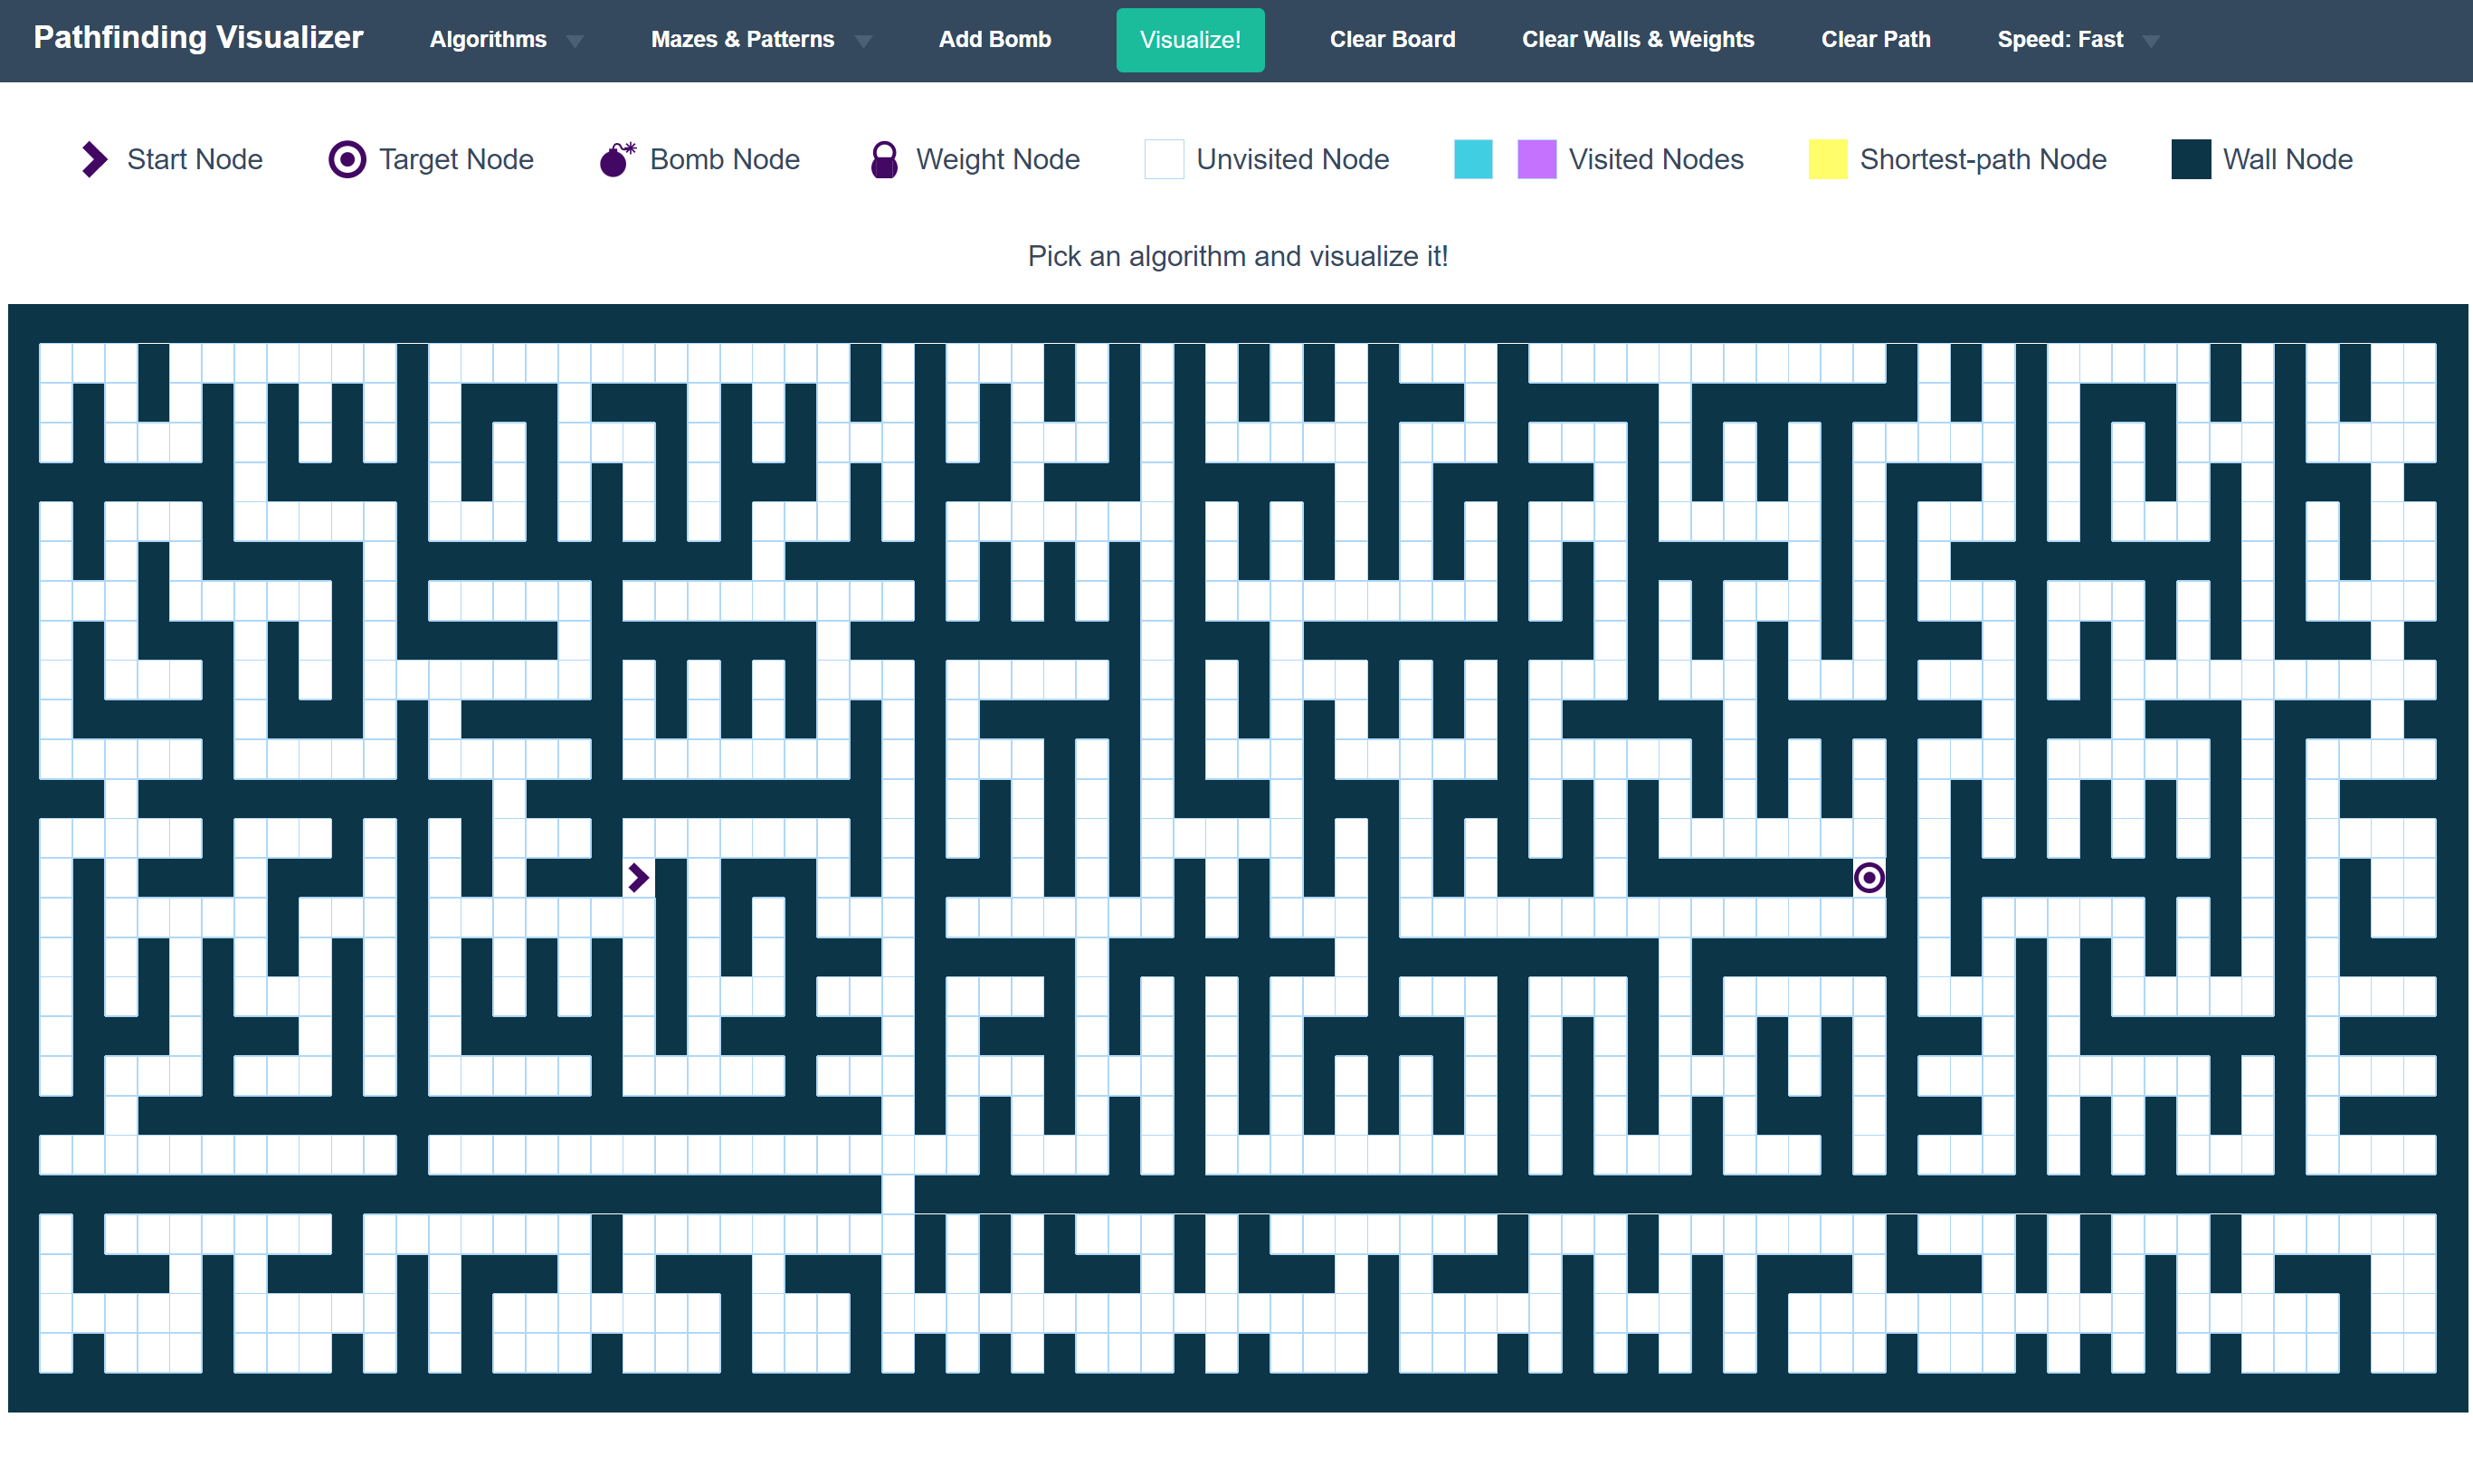
\includegraphics[width=\linewidth]{assets/Existing Solutions/example 1.PNG}
\subparagraph*{pros}
\begin{itemize}
    \item Many different algorithms to choose from.
    \item Start and end nodes can be moved.
    \item Maze can be altered.
    \item If nodes are moved after visualization has run, then the visualization will update.
    \item "Bomb" node, adds a via point that the path must go through.
\end{itemize}
\subparagraph*{cons}
\begin{itemize}
    \item The visualization is too slow.
    \item If maze is altered by user after visualization has run, then the visualization will not update.
\end{itemize}


\paragraph{Example 2}
\href{https://qiao.github.io/PathFinding.js/visual/
}{https://qiao.github.io/PathFinding.js/visual/
}
\newline
In this example, mazes have to be drawn by the user. The maze can then be solved with a number of different algorithms, however, these algorithms have more choice. For example, in the A* option, you can change the heuristic that is used. The available algorithms are:
\begin{itemize}
    \item A*
    \item IDA*
    \item Breadth-First-Search
    \item Best-First-Search
    \item Dijkstra
    \item Jump Point Search
    \item Orthogonal Jump Point Search
    \item Trace
\end{itemize}
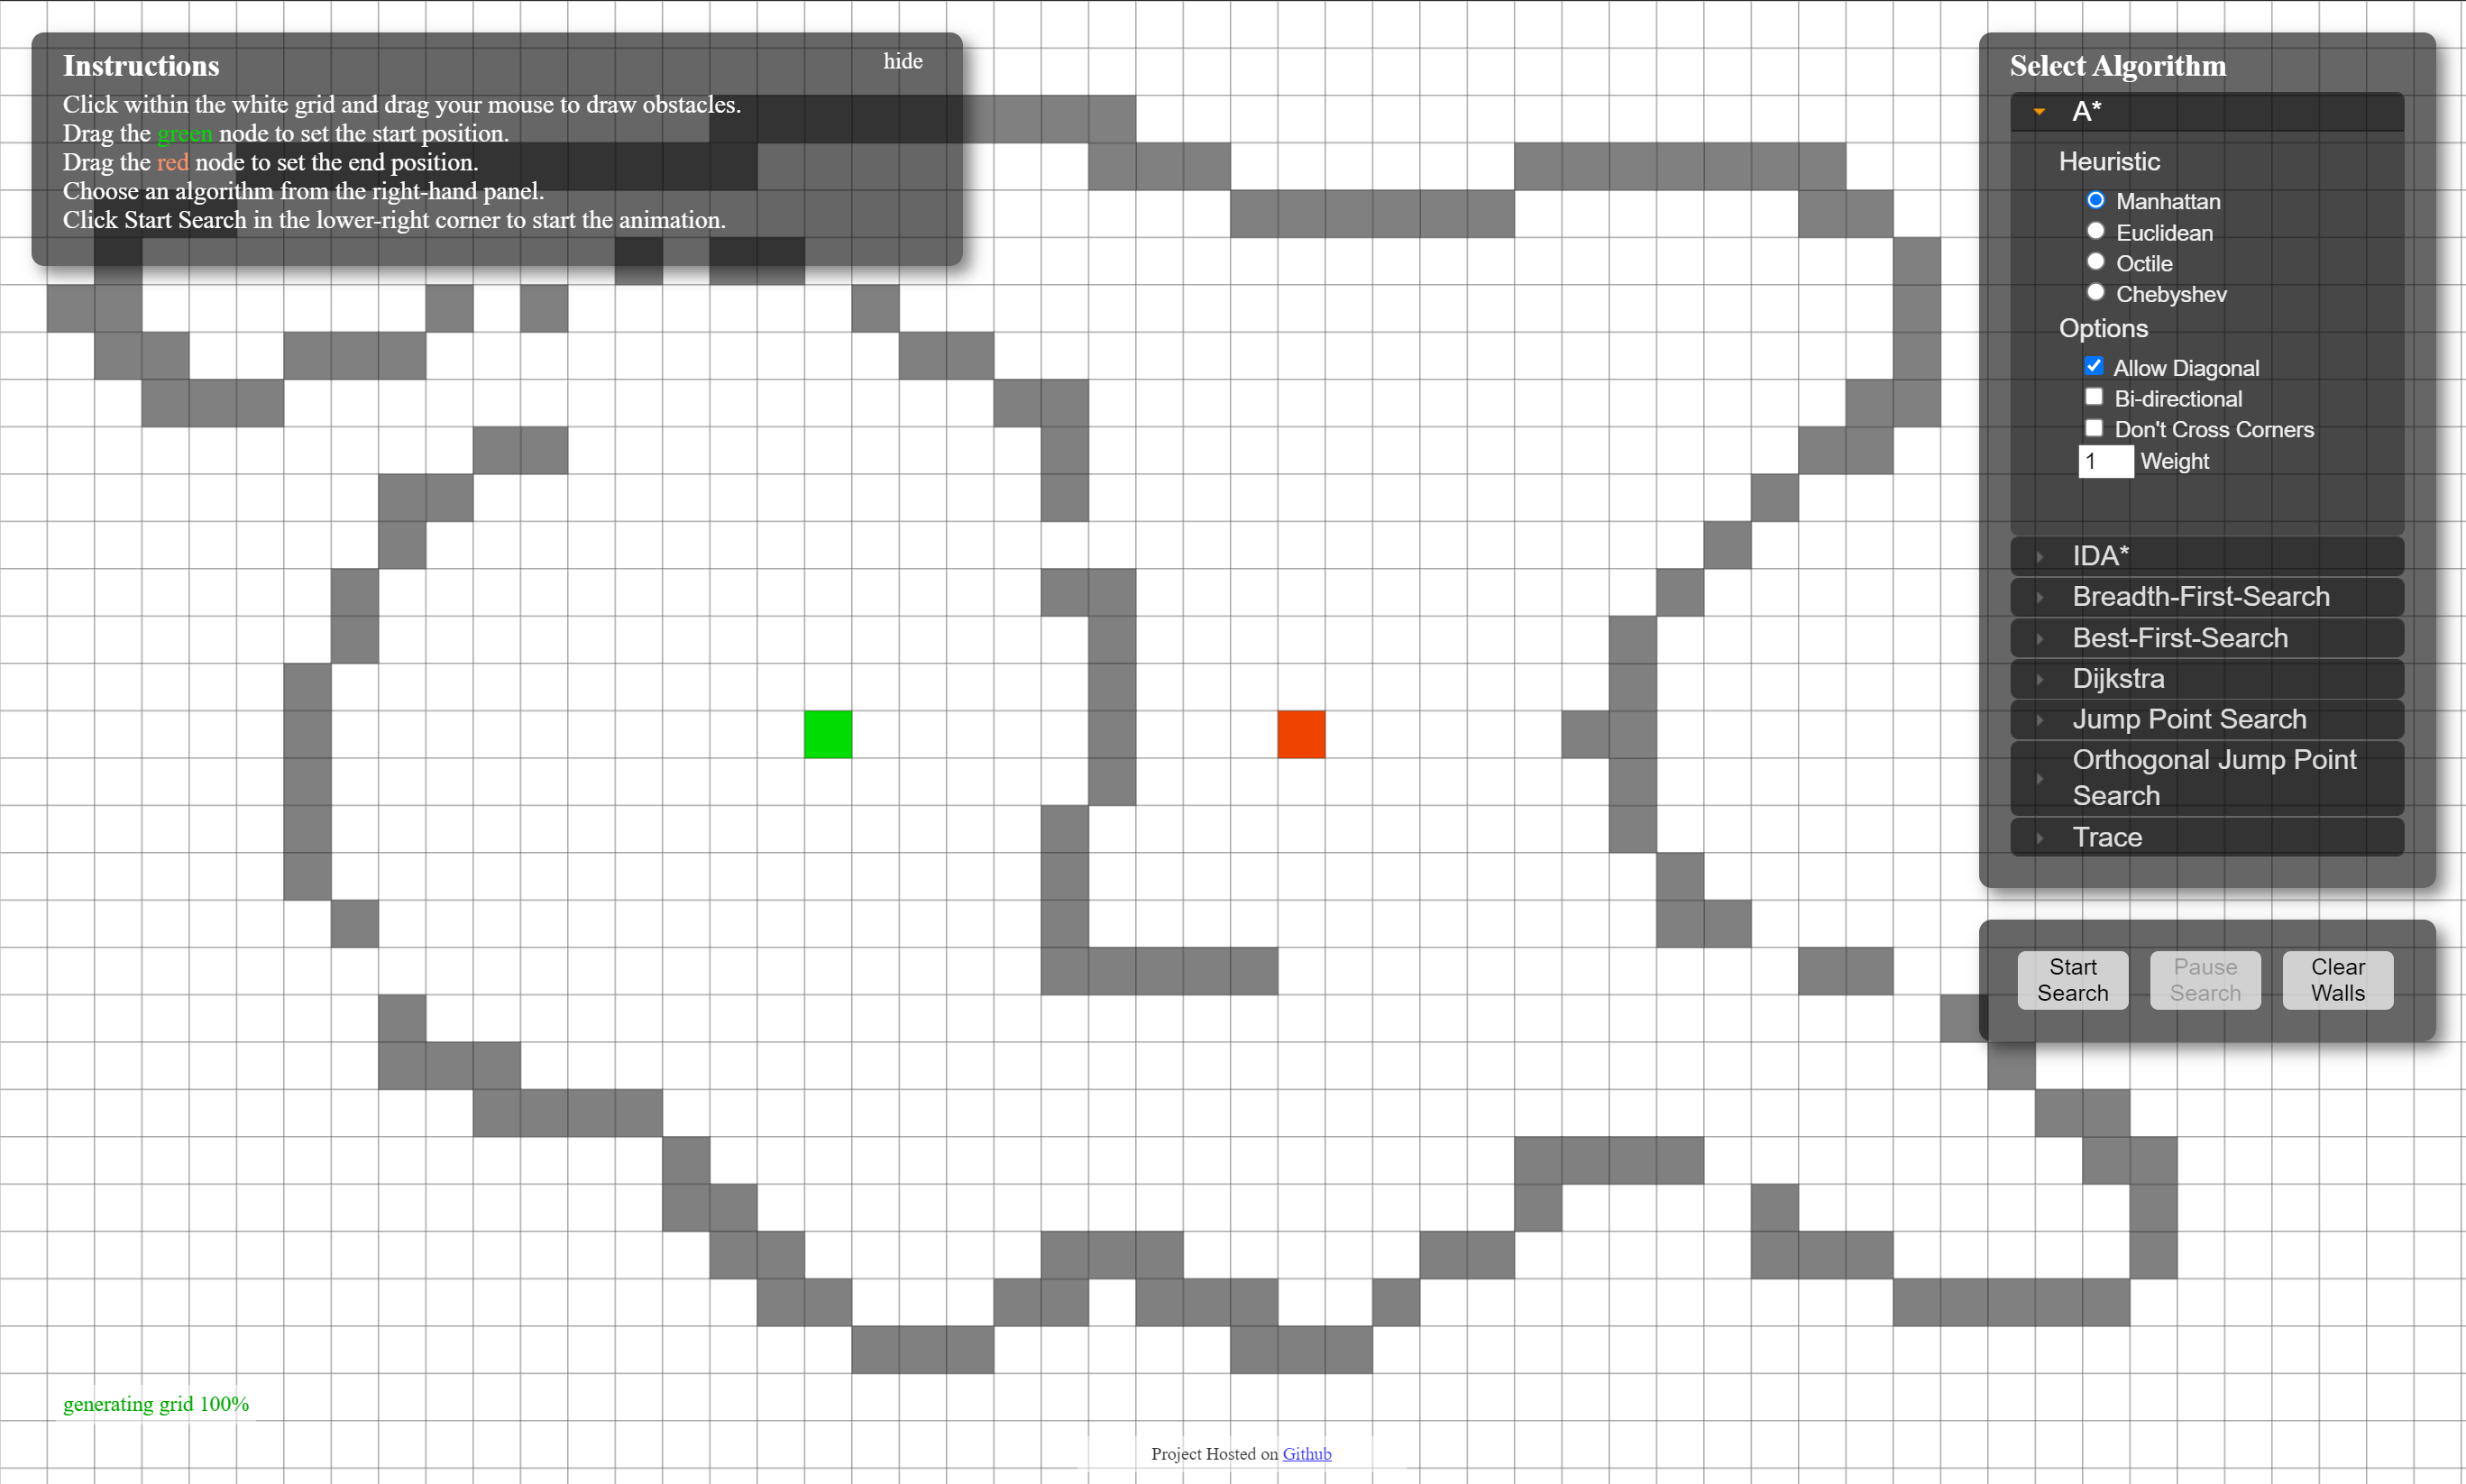
\includegraphics[width=\linewidth]{assets/Existing Solutions/example 2.PNG}
\subparagraph*{pros}
\begin{itemize}
    \item More options to choose from within each algorithm.
\end{itemize}
\subparagraph*{cons}
\begin{itemize}
    \item No maze generation.
    \item Visualization does not update when maze or start/finnish nodes are changed.
\end{itemize}


\paragraph{Example 3}
\href{https://pathfindout.com/
}{https://pathfindout.com/
}
\newline
In this example, mazes can be generated or drawn, however, mazes can only be generated with the recursive division algorithm. There are fewer path finding algorithms to solve the mazes than the others. The available algorithms are:
\begin{itemize}
    \item Dijkstra's Algorithm
    \item A* Search
    \item Breadth First Search
    \item Depth First Search
\end{itemize}
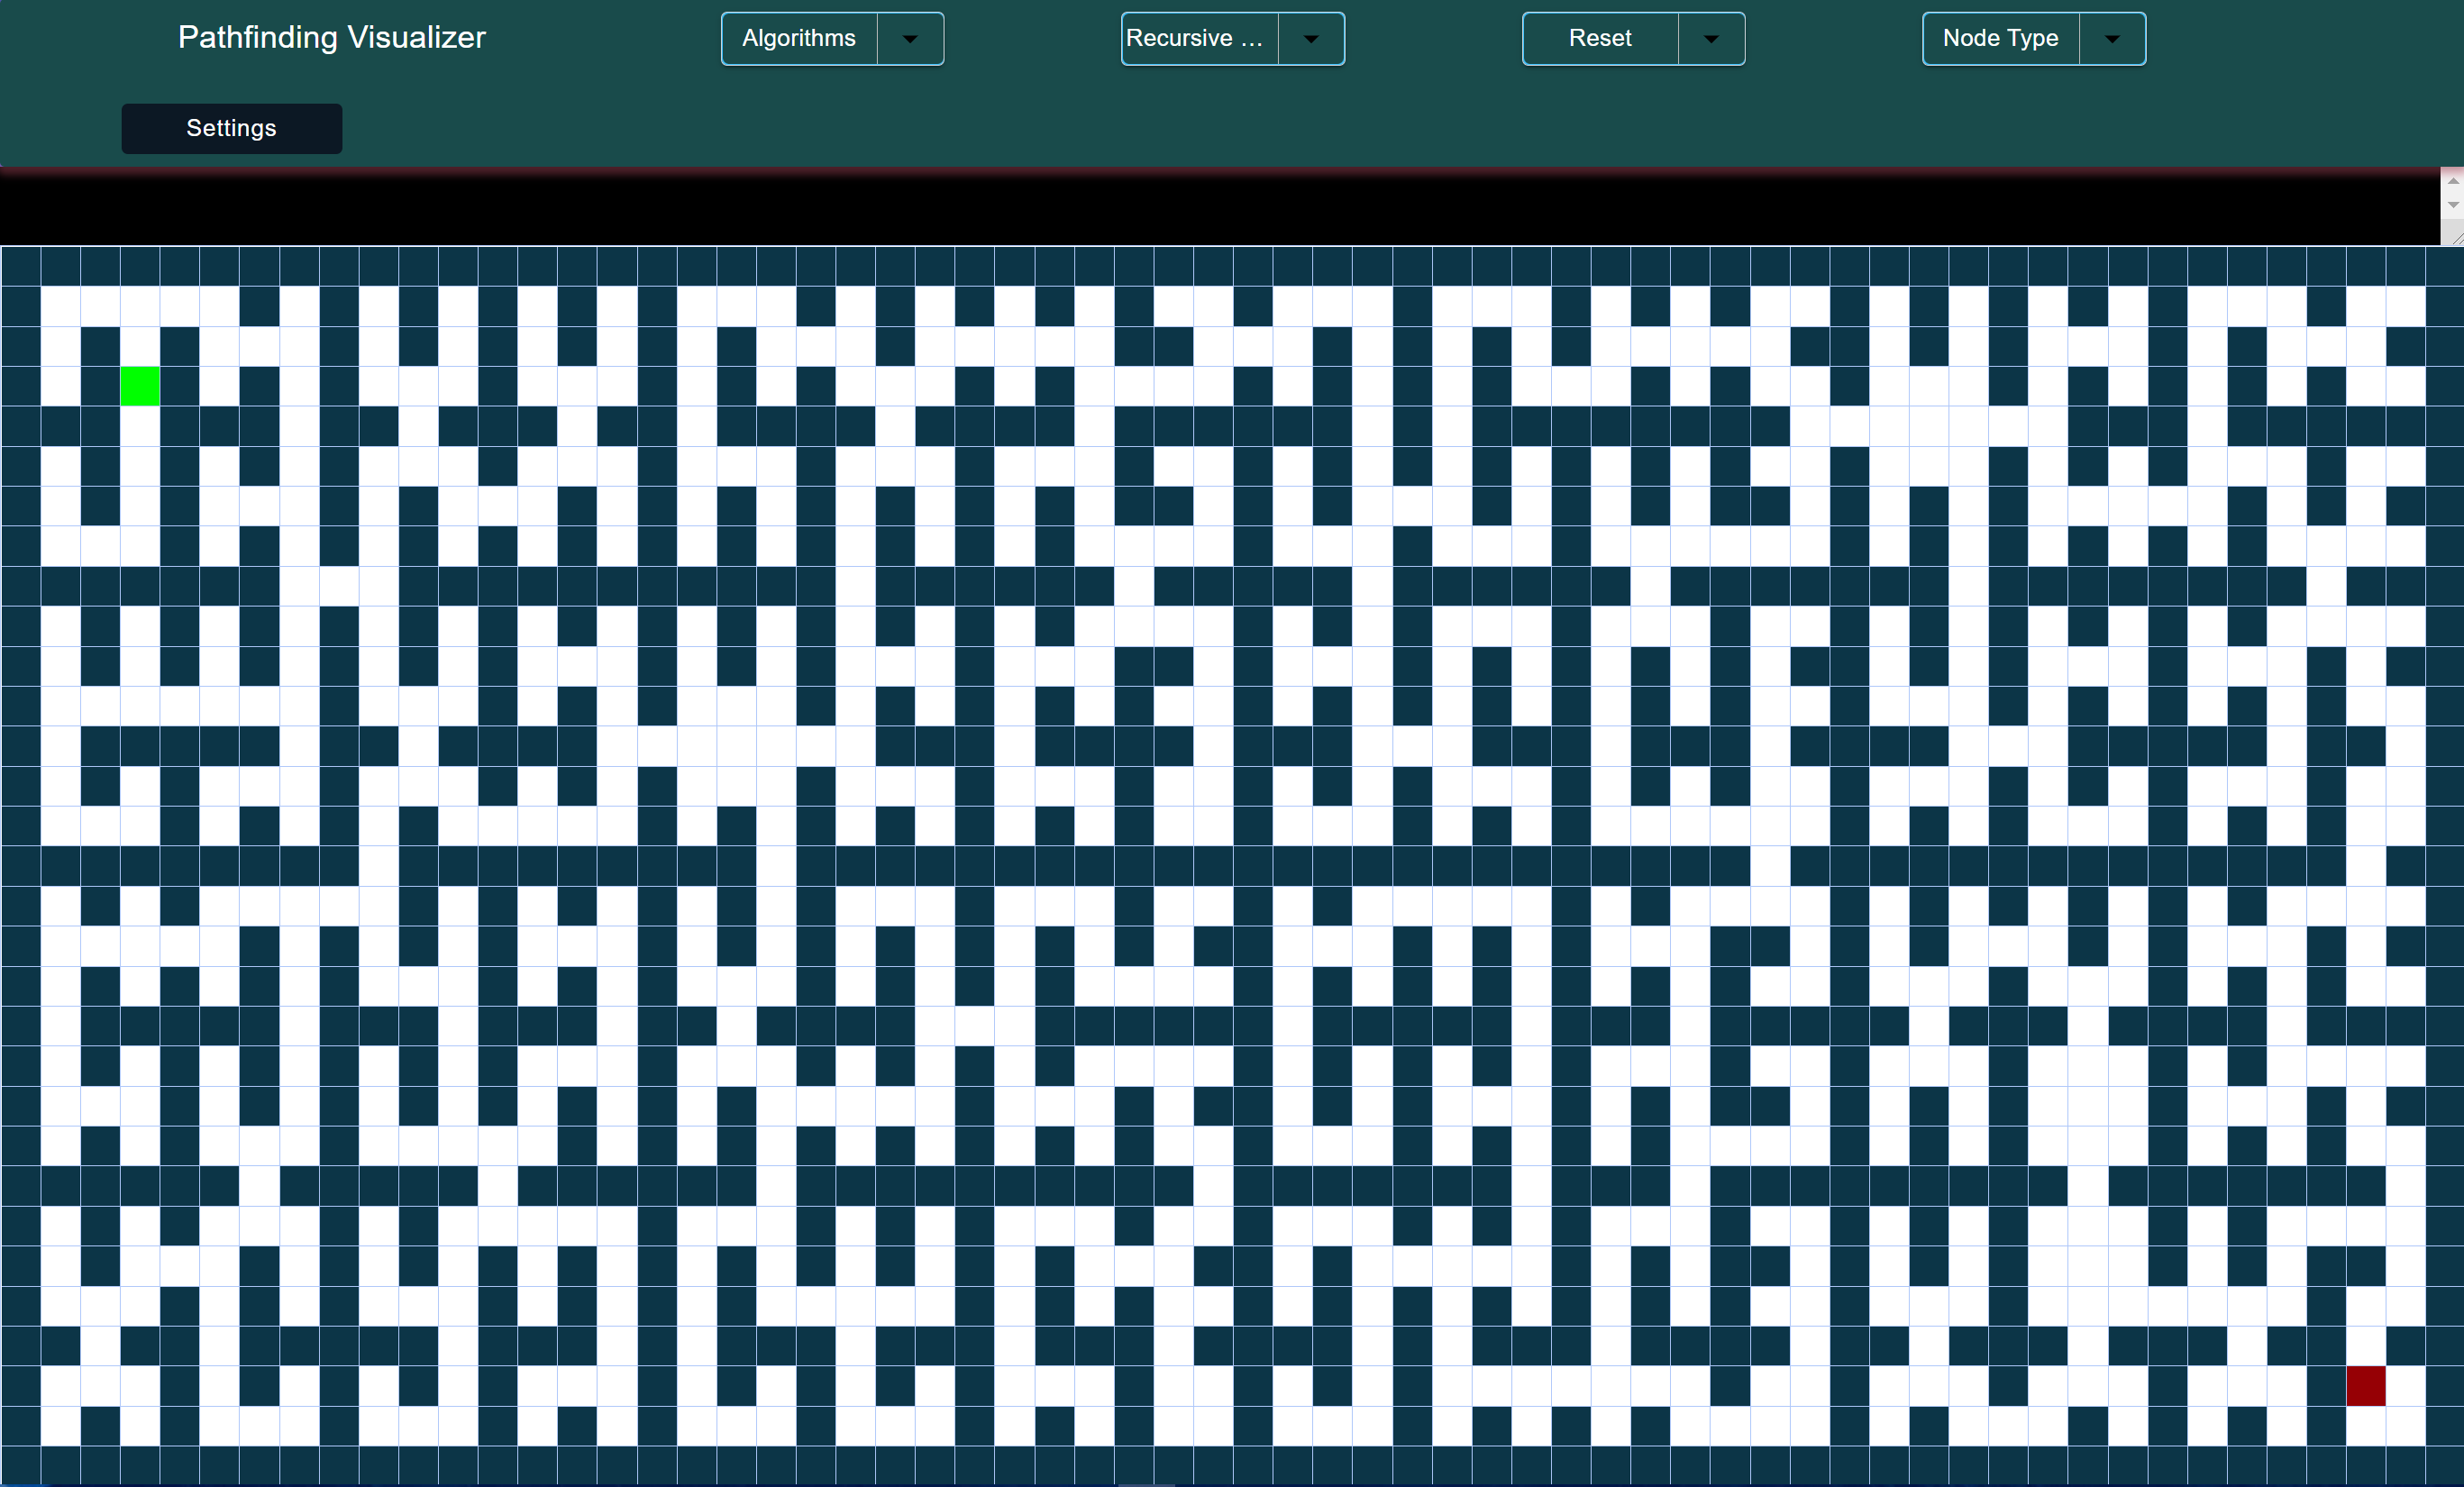
\includegraphics[width=\linewidth]{assets/Existing Solutions/example 3.PNG}
\subparagraph*{pros}
\begin{itemize}
    \item Different weighted nodes available.
    \item Shows how many nodes visited.
    \item Shows final path length.
    \item Data structure for some algorithms can be changed.
    \item Weights of specific node types can be changed.
    \item Node size can be changed.
\end{itemize}
\subparagraph*{cons}
\begin{itemize}
    \item Sometimes generates mazes that cannot be solved.
    \item Cannot edit maze after visualization has run.
    \item Only one maze generation algorithm.
    \item Fewer path finding algorithms to solve the maze.
\end{itemize}

\subsubsection{Proposed Solution}
I will make a path-finding visualization that encompasses as many of the merits of the existing solutions as possible, while also tackling as many of the drawbacks.
\begin{itemize}
    \item Research the different algorithms needed and write the corresponding pseudoscode.
    \item Create a mockup of the user interface.
    \item Create the user interface in react.
    \item Code the algorithms in python.
    \item Create an AWS lambda function in python that runs the algorithms as an API.
    \item Create the react website to visualize the algorithms.
    \item Add additional features suggested by end users.
    \item Test visualization and check that it meets all of the objectives.
\end{itemize}
\subsubsection{Prospective Users}
The users of this system will most likely consist of teachers and students who are learning about path finding algorithms as it will clearly show how the algorithms function.
\paragraph{Questions To Users}
I asked some prospective users some questions about what they would like to see in the visualizer.
\paragraph*{Questions}
\begin{enumerate}
    \item[Q1.]What algorithms would you like to see for maze generation?
    \item[Q2.]What algorithms would you like to see for solving the maze?
    \item[Q3.]What additional features would you like to see in the path finding visualization?
    \item[Q4.]Would it be useful to be able to write your own path finding algorithms that can be run in the visualization?  
\end{enumerate}
\paragraph*{Answers}
\begin{enumerate}
    \item[A1.]I would like to see recursive backtracking and Prim's algorithms used for maze generation, as well as Kruskal's (less important). This is because recursive backtracking and Prims are similar but each has their own advantages and disadvantages and recursive backtracking is different and uses recursion.
    \item[A2.]I would like to see an algorithm(such as Dijkstra's) as well as a heuristic(such as A* or a greedy search), as this will show the difference between a heuristic and an algorithm.
    \item[A3.]Option to add your own png image for the drawing of final path - "a sussy imposter running around the maze".
    \item[A4.]I would find it useful to be able to code my own algorithms. This would allow me to use the visualization with other, lesser known algorithms that I may want to visualize.
\end{enumerate}
The answers to these questions confirms what is required from the visualization, which will be reflected in the objectives. The need for contrasting algorithms is something that I will consider when deciding what algorithms to use.
\subsection{Objectives}
\subsubsection{Generate Mazes}
The website should be able to generate mazes using multiple algorithms, including, but not limited to: Prim's algorithm and recursive backtracking. There should also be a brief description of the algorithm that has been selected.

\subsubsection{Solve Mazes}
The website should be able to solve mazes using multiple algorithms, including, but not limited to: greedy search, Dijkstra's algorithms, depth-first search and breadth-first search. There should also be a brief description of the algorithm that has been selected.

\subsubsection{Customisation}
The user should be able to customize aspects of the visualization, including:
\begin{itemize}
    \item Size of the maze.
    \item Speed of the animation.
    \item The heuristic used in any heuristic algorithms.
\end{itemize}

\subsubsection{User written algorithms}
The website should be able to run algorithms written by the user for both maze generation and solving. This will be done by supplying documentation on what parameters need to be taken in and what will need to be returned from the function for the visualizer to work.

\subsubsection{Update Visualization}
If the start or end nodes are moved once the visualization has been run, then it should update without the user having to rerun the visualization.

\section{Documented Design}
\subsection{Visualization Structure}
The project will be split into two main sections, the first being the visualization and the second being the python API.
The python API will be for generating and solving the mazes, and the react website that will visualize the algorithms. The python API will can be subdivided into two sections, the first being the maze generation and the second being the maze solving. Different parameters will be passed to the API depending on the what the user has requested. These parameters will be:
\begin{itemize}
    \item width
    \item height
    \item type (solve/generate/empty maze)
    \item generate (algorithm for generation)
    \item solve (algorithm for solving)
    \item start
    \item end
\end{itemize} 

When solving the maze, the maze will be sent to the API as part of the body of the request.
\newline
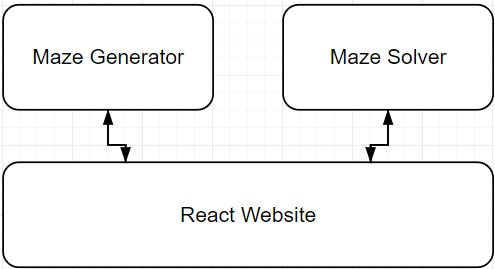
\includegraphics[width=\linewidth]{assets/structure.jpg}
\subsection{User Interaction Flow Chart}
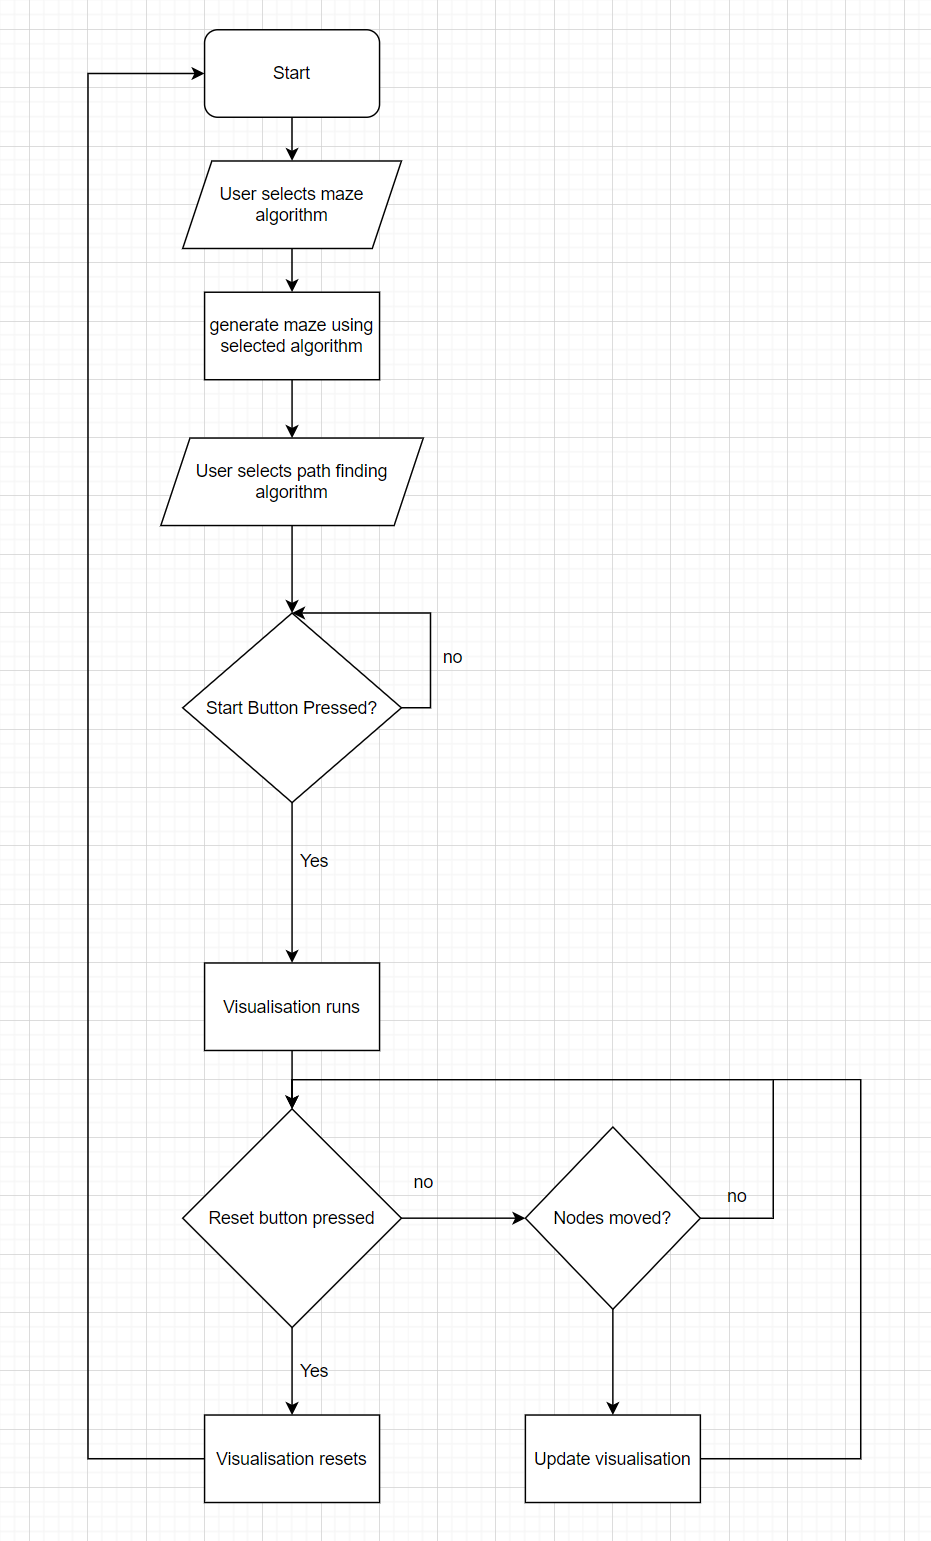
\includegraphics[width=\linewidth, height=17.5cm]{assets/flow chart.PNG}

\subsection{User Interface}
I have used Figma to create a design mockup of how the user interface will look. This allows me to plan what user inputs will be needed.
\newline
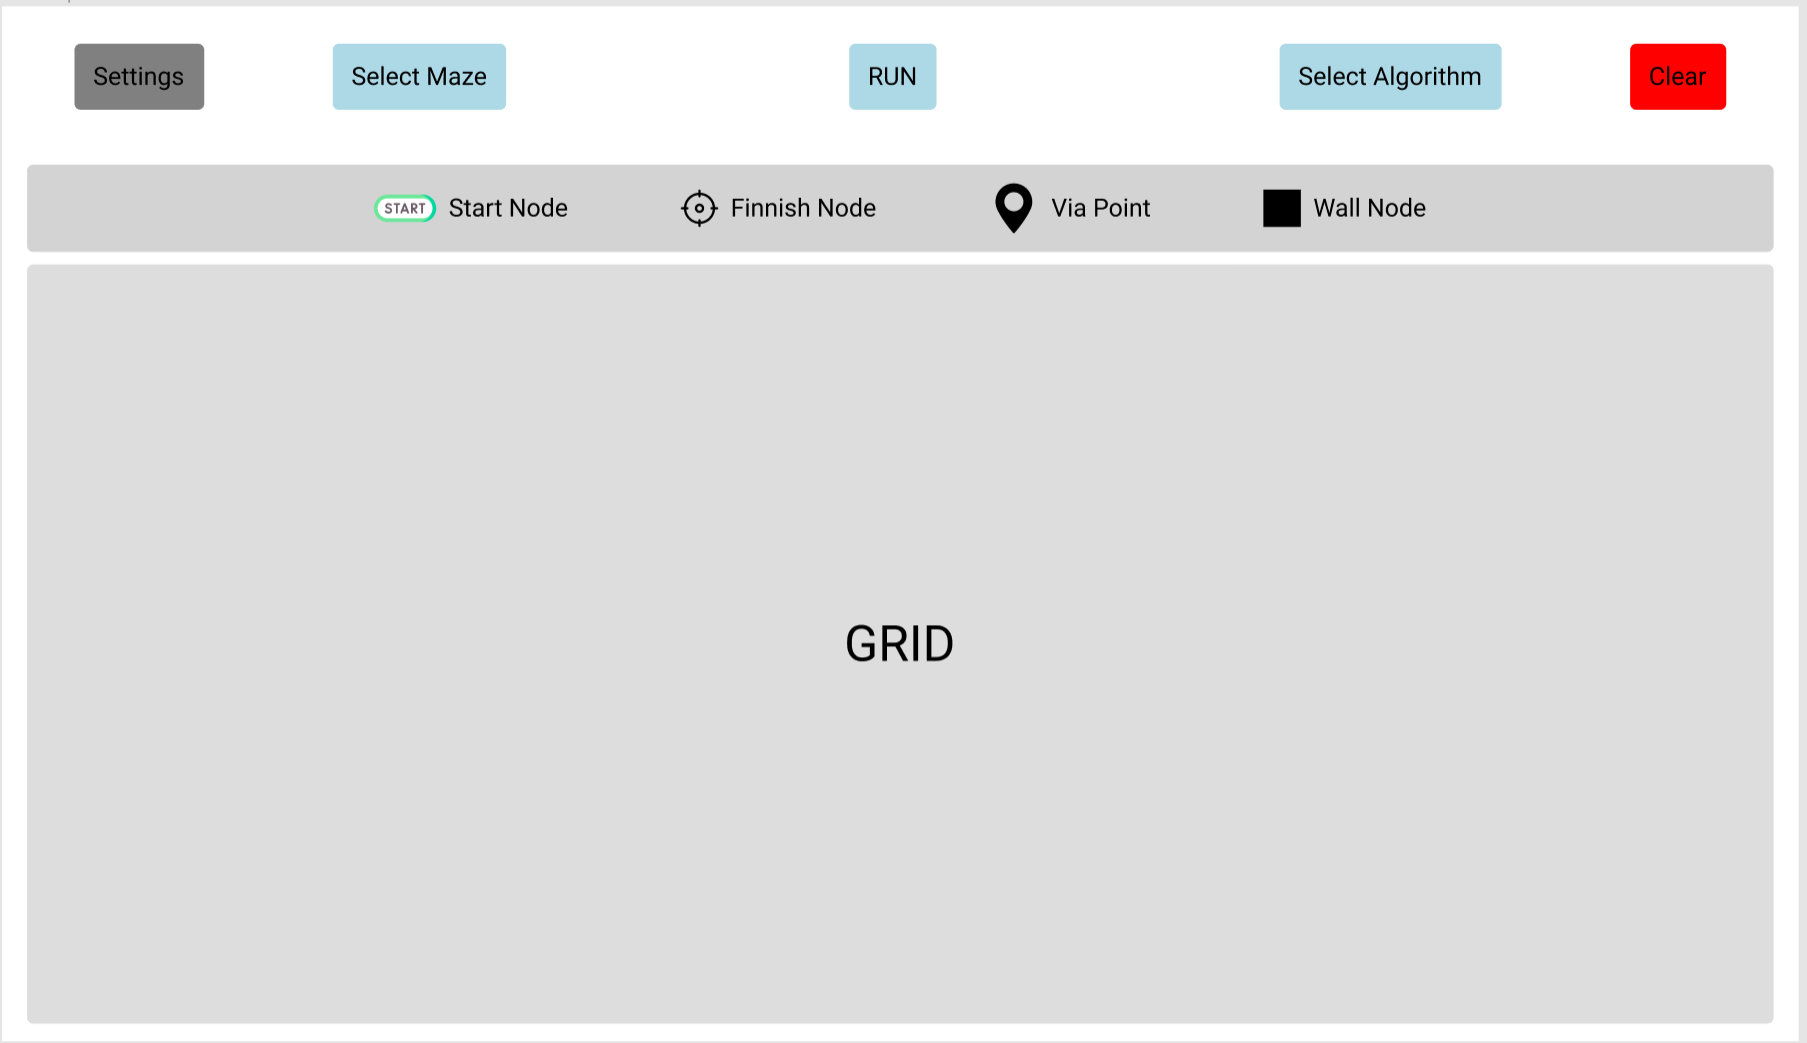
\includegraphics[width=\linewidth]{assets/gui.PNG}
\subsection{Classes Breakdown}

\subsubsection{Genereator}

The generator class will be responsible for generating the maze with different algorithms.
\newline
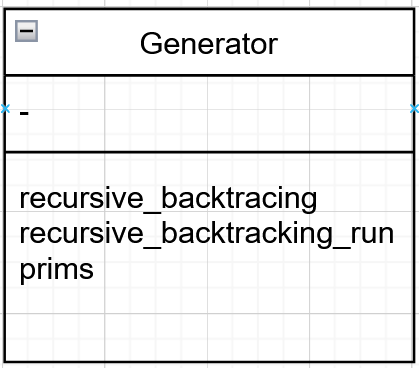
\includegraphics[width=0.5\linewidth]{assets/class diagrams/generator.PNG}

\subsubsection{Solver}

The solver class will be responsible for solving the maze with different algorithms.
\newline
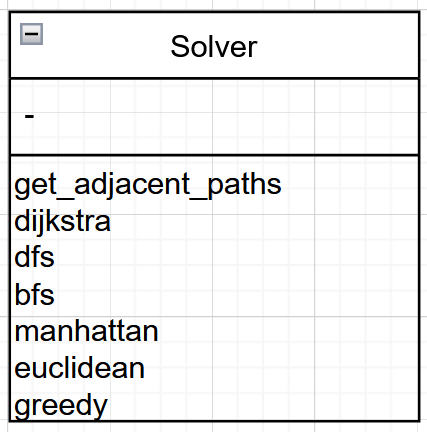
\includegraphics[width=0.5\linewidth]{assets/class diagrams/solver.PNG}

\subsubsection{Maze}

The maze class will be responsible for storing the maze and any other information that is needed, as well as methods for loading a generated maze to be solved and a serialize method for sending the maze to the react app.
\newline
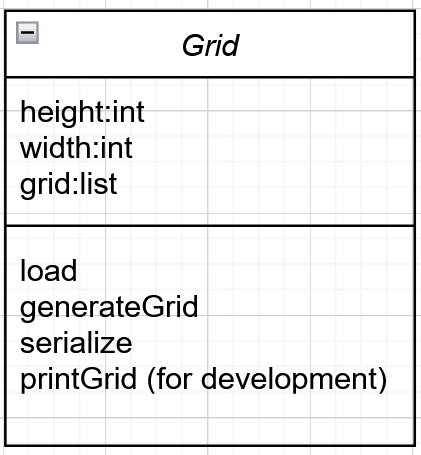
\includegraphics[width=0.5\linewidth]{assets/class diagrams/maze.PNG}

\subsubsection{Node}

The node class will be responsible for storing the nodes and any other information that is needed, as well as methods for loading the nodes from a generated maze and a serialize method for sending the maze to the react app.
\newline
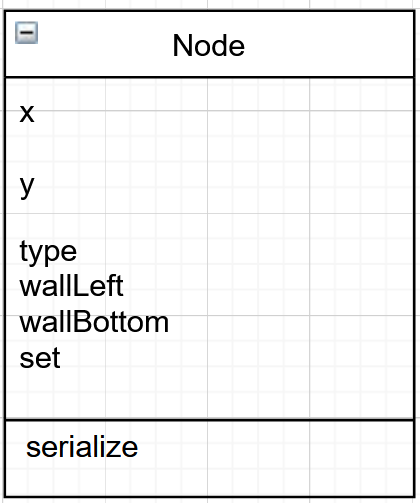
\includegraphics[width=0.5\linewidth]{assets/class diagrams/node.PNG}

\subsection{Algorithms}
\subsubsection{Prims}
Prim's algorithm will have two lists, an inMaze list and a frontier, to store the nodes that are in the maze and in the frontier respectively. To start, the nodes adjacent to the start node will be added to the frontier. Then a random wall will be taken from the frontier, and the wall will be removed from the maze. The node that was connected by removing the wall will then be added to the inMaze list. Any nodes that are adjacent to the new node and not in the maze will be added to the frontier. This will continue while there are nodes in the frontier.

\subsubsection{Recursive Backtracking}
Recursive backtracking will use a stack to store the previous nodes that have been visited. The stack will be a list of Nodes that are added to the stack as they are visited. If the algorithm reaches a node that has no unvisited adjacent nodes, then the algorithm will backtrack to the last node that was visited by popping off of the stack. This will continue until the algorithm backtracks to the start node.

\subsubsection{Dijkstra's}
Dijkstra's algorithm works by keeping a priority queue of the nodes that have not been visited, however, all connections have the same weights, as it is solving a maze. The queue will be a list of Nodes, with their distance initially set to "infinity". The algorithm will then search outwards from the start node, adding the distance from the start to each node as it is discovered, until the end node is reached. The algorithm will then backtrack from the end node to the start node, choosing the node with the lowest distance at each step.

\subsubsection{Depth First Search}
Depth first search(dfs) works by keeping a stack of the nodes that need to be visited, and adding to the stack as new nodes are discovered. When the nodes are added to the stack, the "parent" attribute of the nodes will be updated so that a path can be drawn. If there are no unvisited nodes connected to the current node, then the algorithm will backtrack by popping a node off of the stack. This will continue until the stack is empty or the end node is reached, at which point the algorithm will return and a path will be drawn.

\subsubsection{Breadth First Search}
Breadth first search(bfs) is similar to dfs, however a queue should be used instead of a stack. The queue will be a list of Nodes, with new Nodes being added to the end of the list as they are discovered. When the nodes are added to the queue, the "parent" attribute of the nodes will be updated so that a path can be drawn. The algorithm will keep searching until the queue is empty or the end node is reached, at which point the algorithm will return and a path will be drawn.

\subsubsection{Greedy Search}
Greedy search works by keeping a priority queue, with the heuristic distance from the node to the end node being the priority. The algorithm will start from the start node, searching outwards, adding nodes to the priority queue as they are discovered, with the "parent" attribute being updated so that the path can be drawn. The algorithm will keep searching until the queue is empty or the end node is reached, at which point the algorithm will return and a path will be drawn.
\paragraph*{Heuristic}
Different heuristics can be used for the greedy search. The heuristic I will include are manhattan distance and euclidean distance, as these are some of the most common heuristics.

\subparagraph*{Manhattan Distance}
Manhattan is calculated by
\begin{equation}
    h(n) = |x_{current\ node} - x_{end\ node}| + |y_{current\ node} - y_{end\ node}|
\end{equation}
\subparagraph*{Euclidean Distance}
Euclidean is calculated by
\begin{equation}
    h(n) = \sqrt{(x_{current\ node} - x_{end\ node})^2 + (y_{current\ node} - y_{end\ node})^2}
\end{equation}

\subsection{Subroutine Breakdown API}
\subsubsection{generator.py: recursive\_backtracking}
Parameters:\newline
\indent Grid|2D array of Nodes\newline
Setup the variables for recursive backtracking by creating a list in unvisited nodes.

\subsubsection{generator.py: recursive\_backtracking\_run}
Parameters:\newline
\indent Grid| 2D array of Nodes\newline
\indent unvisited| list of Nodes\newline
\indent current| Node\newline
\indent previous| list of previous Nodes\newline
The recursive backtracking algorithm.

\subsubsection{generator.py: prims}
Parameters:\newline
\indent Grid| 2D array of Nodes\newline
Generate the maze using Prim's algorithm.

\subsubsection{solver.py: get\_adjacent\_paths}
Parameters:\newline
\indent Grid| 2D array of Nodes\newline
\indent node| Node to find adjacent paths\newline
Calculate and return adjacent nodes that are not blocked by walls.

\subsubsection{solver.py: dijkstra}
Parameters:\newline
\indent Grid| 2D array of Nodes\newline
\indent start| Node to start from\newline
\indent end| Node to end at\newline
Use Dijkstra's algorithm to find the shortest path from the start node to the end node and draw a path on the Grid.

\subsubsection{solver.py: dfs}
Parameters:\newline
\indent Grid| 2D array of Nodes\newline
\indent start| Node to start from\newline
\indent end| Node to end at\newline
Use Depth First Search to find the path from the start node to the end node and draw a path on the Grid.

\subsubsection{solver.py: bfs}
Parameters:\newline
\indent Grid| 2D array of Nodes\newline
\indent start| Node to start from\newline
\indent end| Node to end at\newline
Use Breadth First Search to find the path from the start node to the end node and draw a path on the Grid.

\subsubsection{solver.py: manhattan}
Parameters:\newline
\indent node1| Node to calculate distance from\newline
\indent node2| Node to calculate distance to\newline
Calculate and return the manhattan distance between two nodes.

\subsubsection{solver.py: euclidean}
Parameters:\newline
\indent node1| Node to calculate distance from\newline
\indent node2| Node to calculate distance to\newline
Calculate and return the euclidean distance between two nodes.

\subsubsection{solver.py: greedy}
Parameters:\newline
\indent Grid| 2D array of Nodes\newline
\indent start| Node to start from\newline
\indent end| Node to end at\newline
\indent heuristic| function to use for heuristic\newline
Use Greedy Search to find the path from the start node to the end node and draw a path on the Grid.

\subsubsection{grid.py: Node: \_\_init\_\_}
Parameters:\newline
\indent x| x coordinate of node\newline
\indent y| y coordinate of node\newline
\indent type| type of node\newline
Constructor for the Node class.

\subsubsection{grid.py: Node: load}
Parameters:\newline
\indent wallLeft| boolean if there is a wall to the left\newline
\indent wallRight| boolean if there is a wall to the right\newline
Load the walls of the node. Used when loading the maze for solving.

\subsubsection{grid.py: Node: serialize}
Returns the Node as a dictionary to be sent to the react app.

\subsubsection{grid.py: Grid: \_\_init\_\_}
Parameters:\newline
\indent height| height of the maze\newline
\indent width| width of the maze\newline
Constructor for the Grid class.

\subsubsection{grid.py: Grid: load}
Parameters:\newline
\indent grid| 2D array of Nodes\newline
Load the maze into the Grid. Used when loading the maze for solving.

\subsubsection{grid.py: Grid: serialize}
Returns the Grid as a dictionary to be sent to the react app.


\subsubsection{grid.py: Grid: generateGrid}
Generate an empty grid.

\subsubsection{grid.py: Grid: printGrid}
Print the grid, used when developing maze generation and solving algorithms.

\subsection{Subroutine Breakdown react app}
\subsubsection{App.js: App: Constructor}
Parameters:\newline
\indent props| props passed from react\newline
Constructor for the App class.

\subsubsection{App.js: App: componentDidMount}
Method runs when the component mounts in the DOM, used to load an empty maze when the app loads.

\subsubsection{App.js: App: setHeuristic}
Parameters:\newline
\indent heuristic| heuristic to use\newline
Callback function to change the heuristic used for the greedy search from the settings component.

\subsubsection{App.js: App: setSpeed}
Parameters:\newline
\indent speed| speed to use\newline
Callback function to change the speed of the maze generation from the settings component.

\subsubsection{App.js: App: setSize}
Parameters:\newline
\indent size| size to use\newline
Callback function to change the size of the maze from the settings component, the maze is reset when the size is changed.

\subsubsection{App.js: App: setStart}
Parameters:\newline
\indent start| start node to use\newline
Callback function to change the start node of the maze when the start node is dragged and dropped to a new location.

\subsubsection{App.js: App: setEnd}
Parameters:\newline
\indent end| end node to use\newline
Callback function to change the end node of the maze when the end node is dragged and dropped to a new location.

\subsubsection{App.js: App: setAlgorithm}
Parameters:\newline
\indent algorithm| algorithm to use for generating the maze\newline
Callback function to change the algorithm used to generate the maze from the settings component.

\subsubsection{App.js: App: setSolve}
Parameters:\newline
\indent algorithm| algorithm to use for solving the maze\newline
Callback function to change the algorithm used to solve the maze from the settings component.

\subsubsection{App.js: App: async should\_solve}
Method to check if the maze should ber resolved after start or end nodes have moved, and if it should be resolved, then resolve the maze. This method is asynchronous, as it changes the state of the app, which is an asynchronous operation and must be awaited before continuing.

\subsubsection{App.js: App: async clear\_node\_index}
Method to clear the index of the nodes so that the maze can be solved again. This method is asynchronous, as it changes the state of the app, which is an asynchronous operation and must be awaited before continuing, and it returns a promise, which is resolved once the state has been updated.

\subsubsection{App.js: App: async fetchGrid}
Method to fetch the maze from the server. This method is asynchronous, as it changes the state of the app and is making a call to the API over the internet, both of which are asynchronous operations and must be awaited before continuing.

\subsubsection{App.js: App: async solveGrid}
Method to send the grid to the API to be solved and receive a response with a solved maze. This method is asynchronous, as it changes the state of the app and is making a call to the API over the internet, both of which are asynchronous operations and must be awaited before continuing.

\subsubsection{App.js: App: async clearGrid}
Method to get an empty grid from the API. This method is asynchronous, as it changes the state of the app and is making a call to the API over the internet, both of which are asynchronous operations and must be awaited before continuing.

\subsubsection{App.js: App: render}
Method to render the react component.

\subsubsection{DisplayGrid.jsx: DisplayGrid: handelDrop}
Parameters:\newline
\indent pos| position of the node that is dropped\newline
Callback function to handle the drop of a start or end node.

\subsubsection{DisplayGrid.jsx: DisplayGrid: setDragObject}
Parameters:\newline
\indent type| type of node that is being dragged\newline
Callback function to set the type of node that is being dragged.

\subsubsection{DisplayGrid.jsx: DisplayGrid: renderTable}
Method to render the table of the grid.

\subsubsection{DisplayGrid.jsx: DisplayGrid: render}
Method to render the react component. It will return a table of the grid if there is a grid, else it will show a message saying that there is no grid.

\subsubsection{DisplayNode.jsx: DisplayNode: handelDragStart}
Callback function to handle the start of the node being dragged. It will set the type of node being dragged to the type of node that is being dragged in the parent component using DisplayGrid.jsx: DisplayGrid: setDragObject.

\subsubsection{DisplayNode.jsx: DisplayNode: handelDrop}
Callback function to handle the drop of the node.

\subsubsection{DisplayNode.jsx: DisplayNode: handelDragOver}
Callback function to run when the node is dragged over this node. It will change the colour of the node to indicate that it is being dragged over.

\subsubsection{DisplayNode.jsx: DisplayNode: handelDragLeave}
Callback function to run when the node is dragged off this node. It will change the colour of the node to indicate that it is no longer being dragged over.

\subsubsection{DisplayNode.jsx: DisplayNode: render}
Method to render the react component. Selection is used to examine the props and apply the correct attributes to the node.

\subsubsection{Settings.jsx: Settings: componentDidMount}
Method to run when the component mounts in the DOM. It will add an event listener to the document to detect if the user clicks outside the settings component.

\subsubsection{Settings.jsx: Settings: componentWillUnmount}
Method to run when the component is unmounted from the DOM. It will remove the event listener from the document.

\subsubsection{Settings.jsx: Settings: handelClickOutsize}
Parameters:\newline
\indent event| event that is triggered when the user clicks outside the settings component\newline
Callback function to handle the click outside the settings component.

\subsubsection{Settings.jsx: Settings: handelSizeChange}
Parameters:\newline
\indent event| event that is triggered when the user changes the size of the maze\newline
Callback function to the change of the size of the maze in the parent component using App.jsx: App: setSize.

\subsubsection{Settings.jsx: Settings: setHeuristic}
Parameters:\newline
\indent heuristic| selected heuristic\newline
Callback function to change the heuristic used for the greedy search in the parent component using App.jsx: App: setHeuristic.

\subsubsection{Settings.jsx: Settings: renderSettings}
Method to render the settings component if the settings button is clicked.

\section{Technical Solution}
A running solution of the project is available at \url{https://olivertemple.github.io/nea/}.
\subsection{Summary Of Skills Used}
These tables are a list of some of the skills I have used in this project, with line numbers of where they are demonstrated.
\begin{center}
    
    \begin{tabular}{ |p{0.4\linewidth}|p{0.8\linewidth}| }
        \hline
        Skill & Where to find \\
        \hline
        \hline
        Stacks & Solver.py: dfs \\
        \hline
        Queues & Solver.py: bfs, Solver.py: dijkstra\\
        \hline
        Priority Queue & Solver.py: greedy \\
        \hline
        Recursive Algorithms & Generator.py: recursive\_backtracking\_run \\
        \hline
        Complex OOP & grid.py: Grid, grid.py: Node, App.js, DisplayGrid.jsx, DisplayNode.jsx, Settings.jsx,  \\
        \hline
        Dynamic generation of objects & Grid.py: Grid: generateGrid \\
        \hline
        Client-server model, parsing JSON & Called from App.js: 117, App.js: 131, App.js: 151, request handled in lambda\_function.py \\
        \hline
        Dictionaries & lambda\_function.py, grid.py: Grid: serialize, grid.py: Node: serialize \\
        \hline
        Multi-dimensional arrays & grid.py (used to store grid), generator.py: prims (inMaze, frontier) \\
        \hline 
        Simple mathematical calculations & solver.py: manhattan, solver.py: euclidean \\
        \hline
        Complex Algorithms & solver.py, generator.py \\
        \hline
        GUI & App.js, DisplayGrid.jsx, DisplayNode.jsx, Footer.jsx, GeneratorInfo.jsx, Menu.jsx, MenuKey.jsx, Settings.jsx, SolverInfo.jsx \\
        \hline
        Graph traversals & solver.py, generator.py \\
        \hline
    \end{tabular}

\end{center}

\subsection{The Full Code}

\subsubsection{Python API: lambda\_function.py}
\lstinputlisting[language=python, linewidth=1.3\linewidth]{../python api/lambda_function.py}

\subsubsection{Python API: grid.py}
\lstinputlisting[language=python, linewidth=1.3\linewidth]{../python api/grid.py}

\subsubsection{Python API: generator.py}
\lstinputlisting[language=python, linewidth=1.3\linewidth]{../python api/generator.py}

\subsubsection{Python API: solver.py}
\lstinputlisting[language=python, linewidth=1.3\linewidth]{../python api/solver.py}

\subsubsection{React App: App.js}
\lstinputlisting[language=JavaScript, linewidth=1.3\linewidth]{../react app/src/App.js}

\subsubsection{React App: Menu.jsx}
\lstinputlisting[language=JavaScript, linewidth=1.3\linewidth]{../react app/src/components/Menu.jsx}

\subsubsection{React App: MenuKey.jsx}
\lstinputlisting[language=JavaScript, linewidth=1.3\linewidth]{../react app/src/components/MenuKey.jsx}

\subsubsection{React App: DisplayGrid.jsx}
\lstinputlisting[language=JavaScript, linewidth=1.3\linewidth]{../react app/src/components/DisplayGrid.jsx}

\subsubsection{React App: DisplayNode.jsx}
\lstinputlisting[language=JavaScript, linewidth=1.3\linewidth]{../react app/src/components/DisplayNode.jsx}

\section{Testing}
To test the project as a whole, I will check the following:
\begin{enumerate}
    \item[Test1.] Load the react app and check that and empty maze is generated correctly.
    \item[Test2.] Change the size of the maze and check that the size changes and doesn't go below 1.
    \item[Test3.] Run each of the maze generation algorithms and check that the maze is generated correctly and is solvable.
    \item[Test4.] Solve an assortment of mazes with assorted sizes using each of the algorithms (including heuristics for the greedy search) and check that they run correctly.
    \item[Test5.] Use different speeds when solving the mazes and check that the speed changes correctly.
    \item[Test6.] Reset the maze and check that the maze is reset correctly.
    \item[Test7.] Drag and drop the start and finnish nodes. Check that the maze resolves correctly. 
\end{enumerate}

\subsection{Test1: Pass}
Upon loading the react app, an empty maze is generated.
\newline
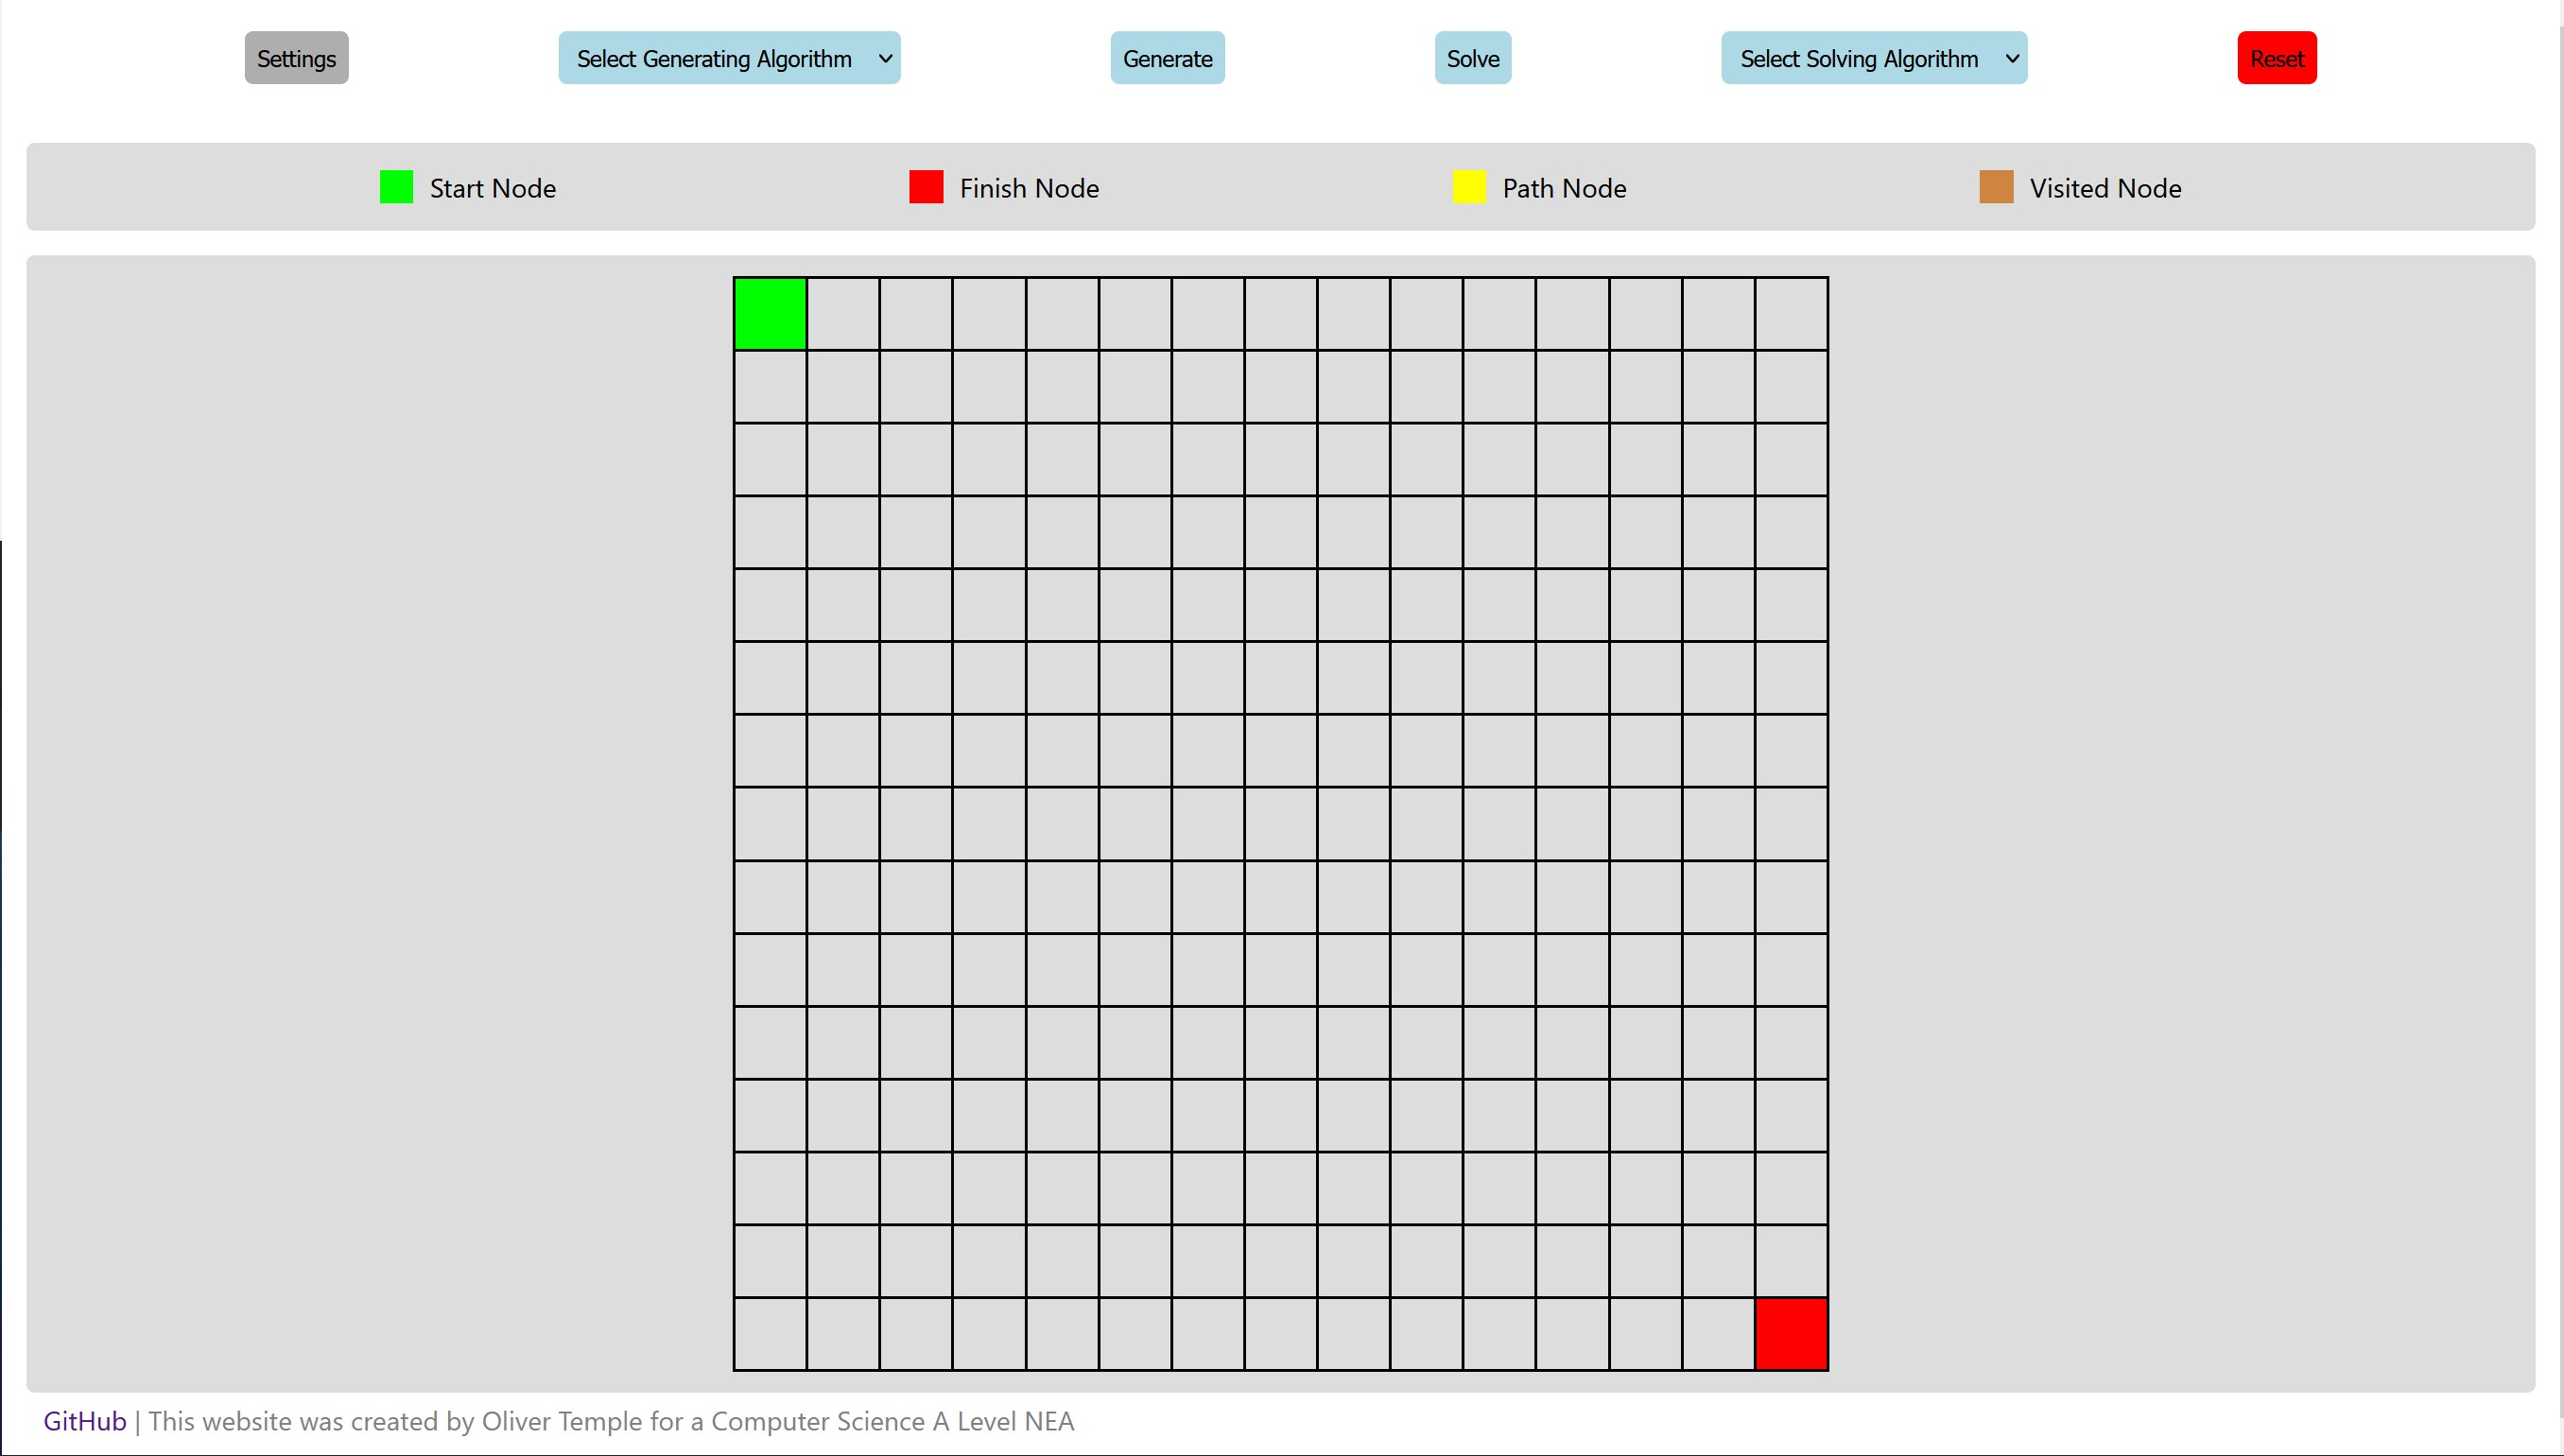
\includegraphics[width=\linewidth]{assets/testing/test1.jpg}

\subsection{Test2: Pass}
The size can be changed down to 1 and the maze is still generated correctly, you cannot go blow 1.
\newline
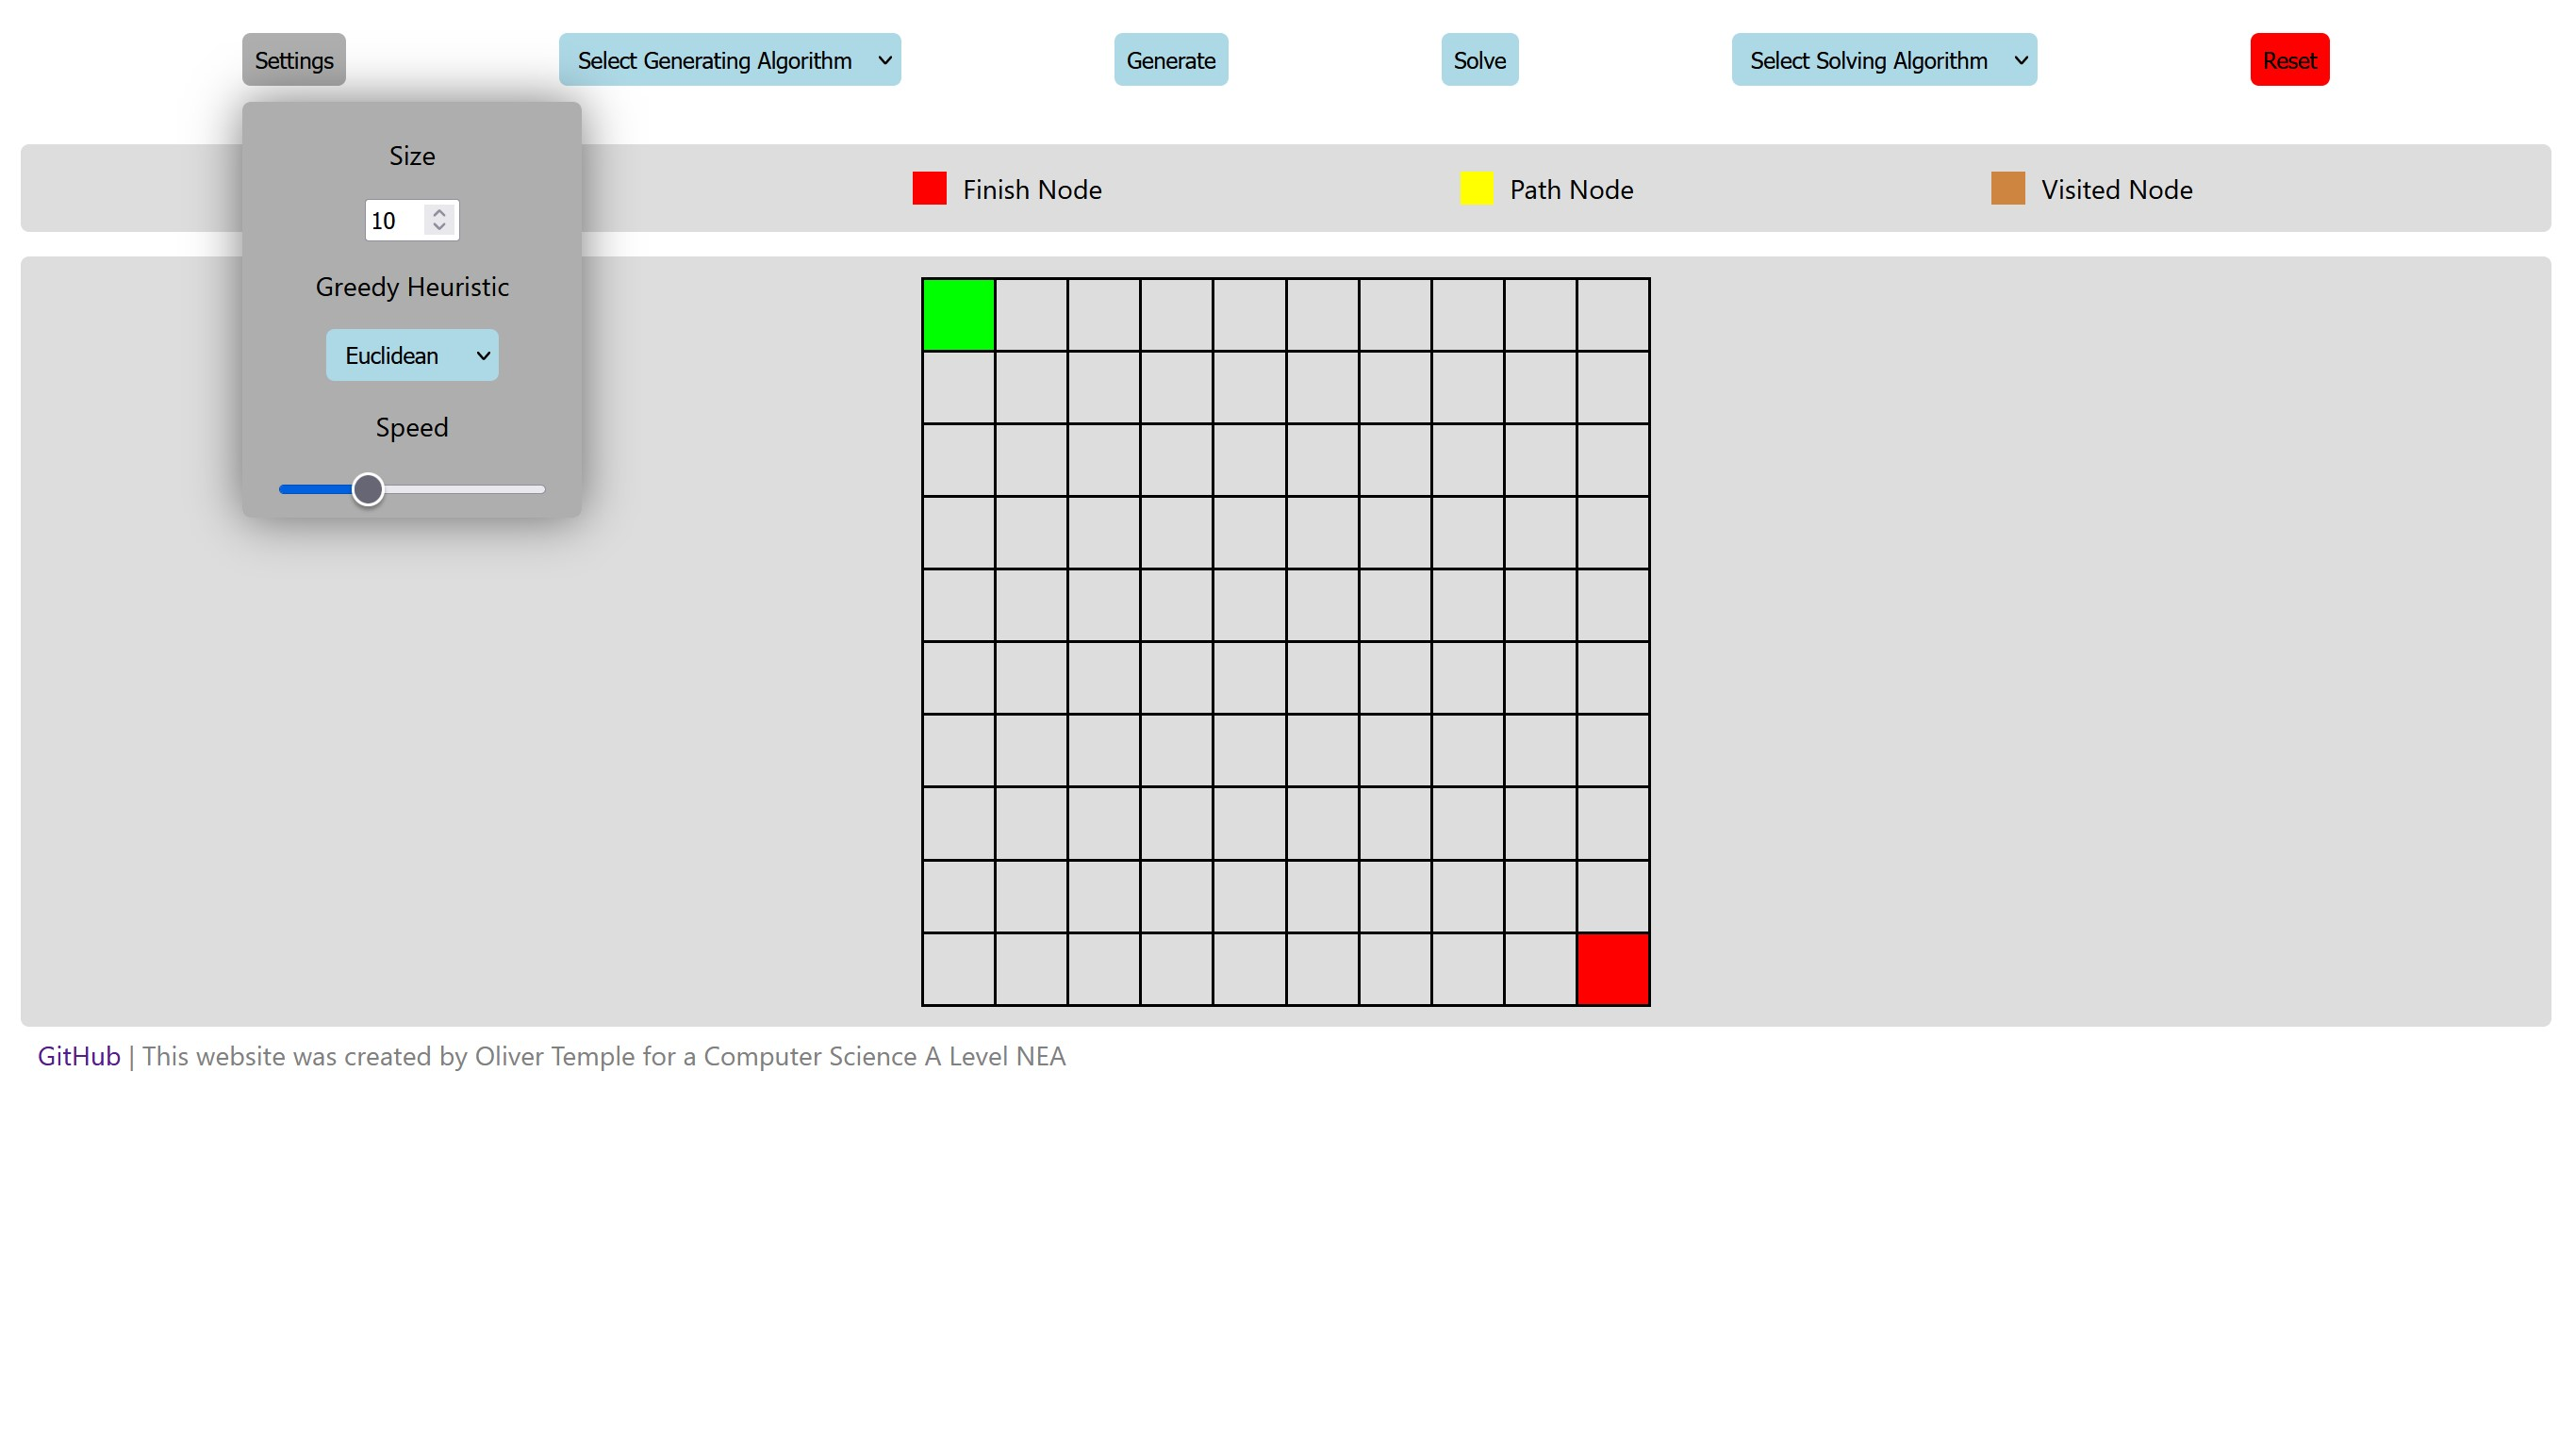
\includegraphics[width=\linewidth]{assets/testing/test2a.jpg}
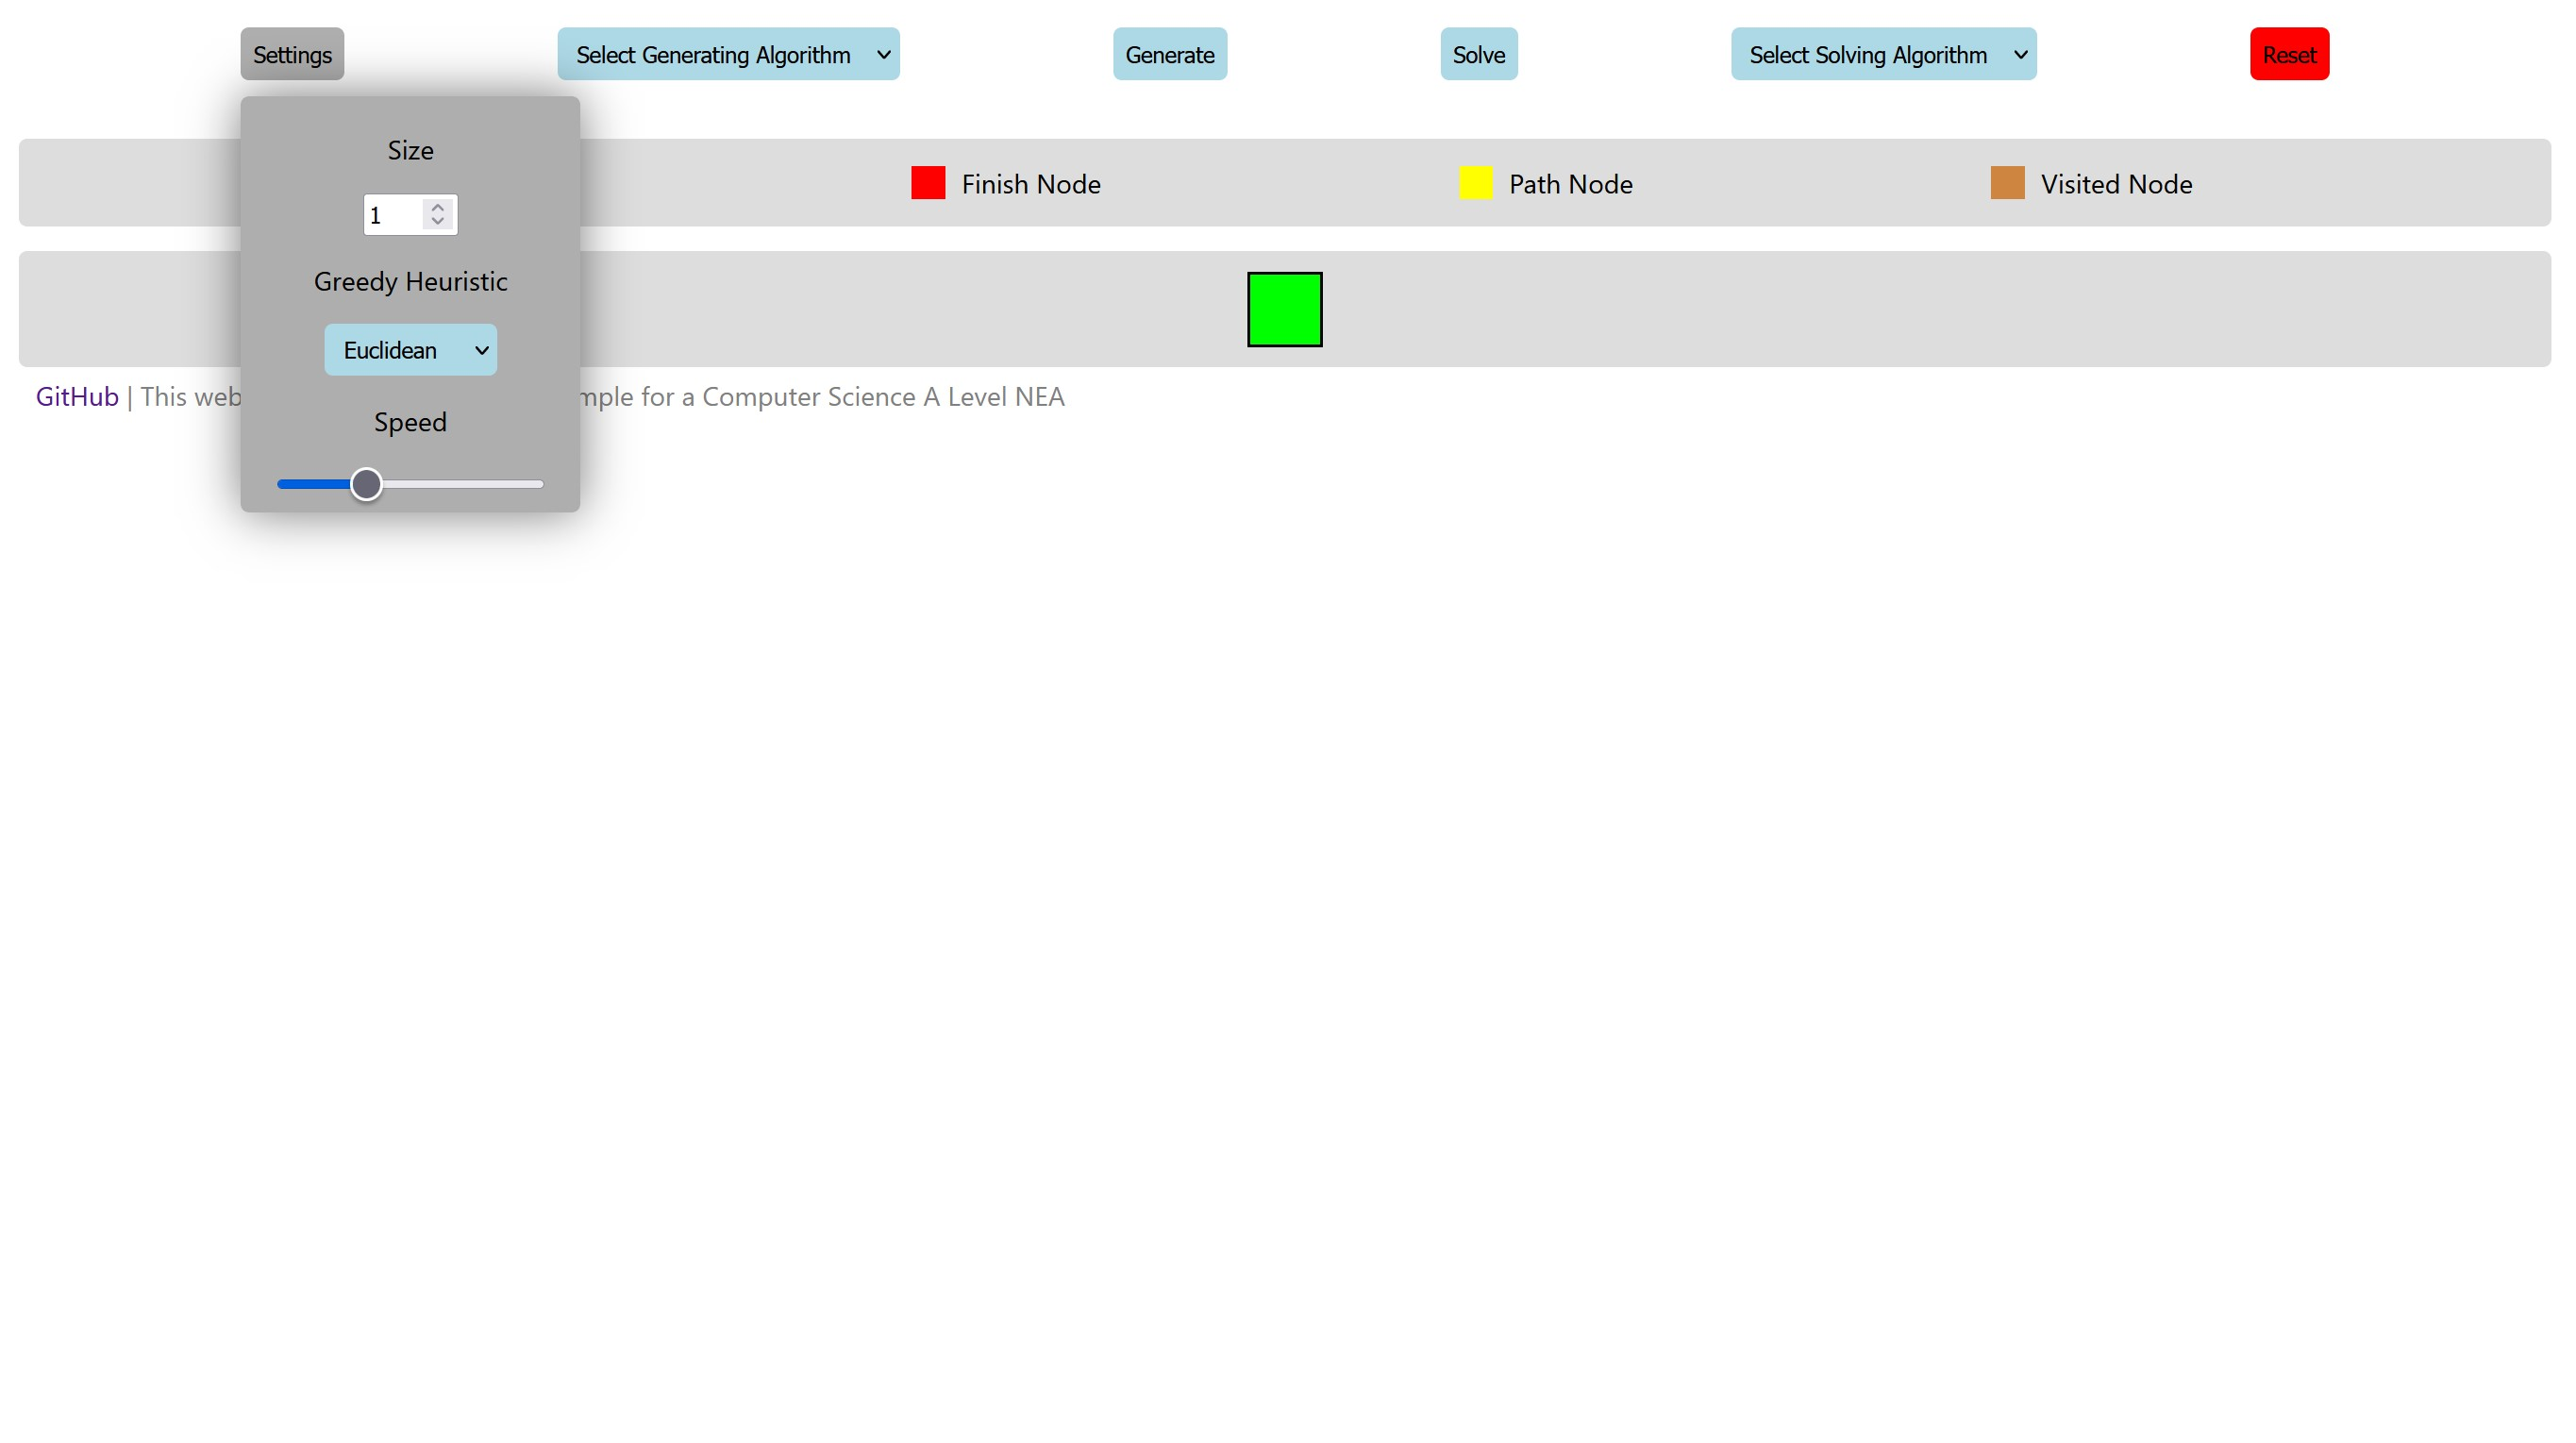
\includegraphics[width=\linewidth]{assets/testing/test2b.jpg}

\subsection{Test3: Pass}
Blow are screenshots of a maze being generated using each of the different algorithms, with different size mazes.
\subsubsection{Prim's Algorithm}
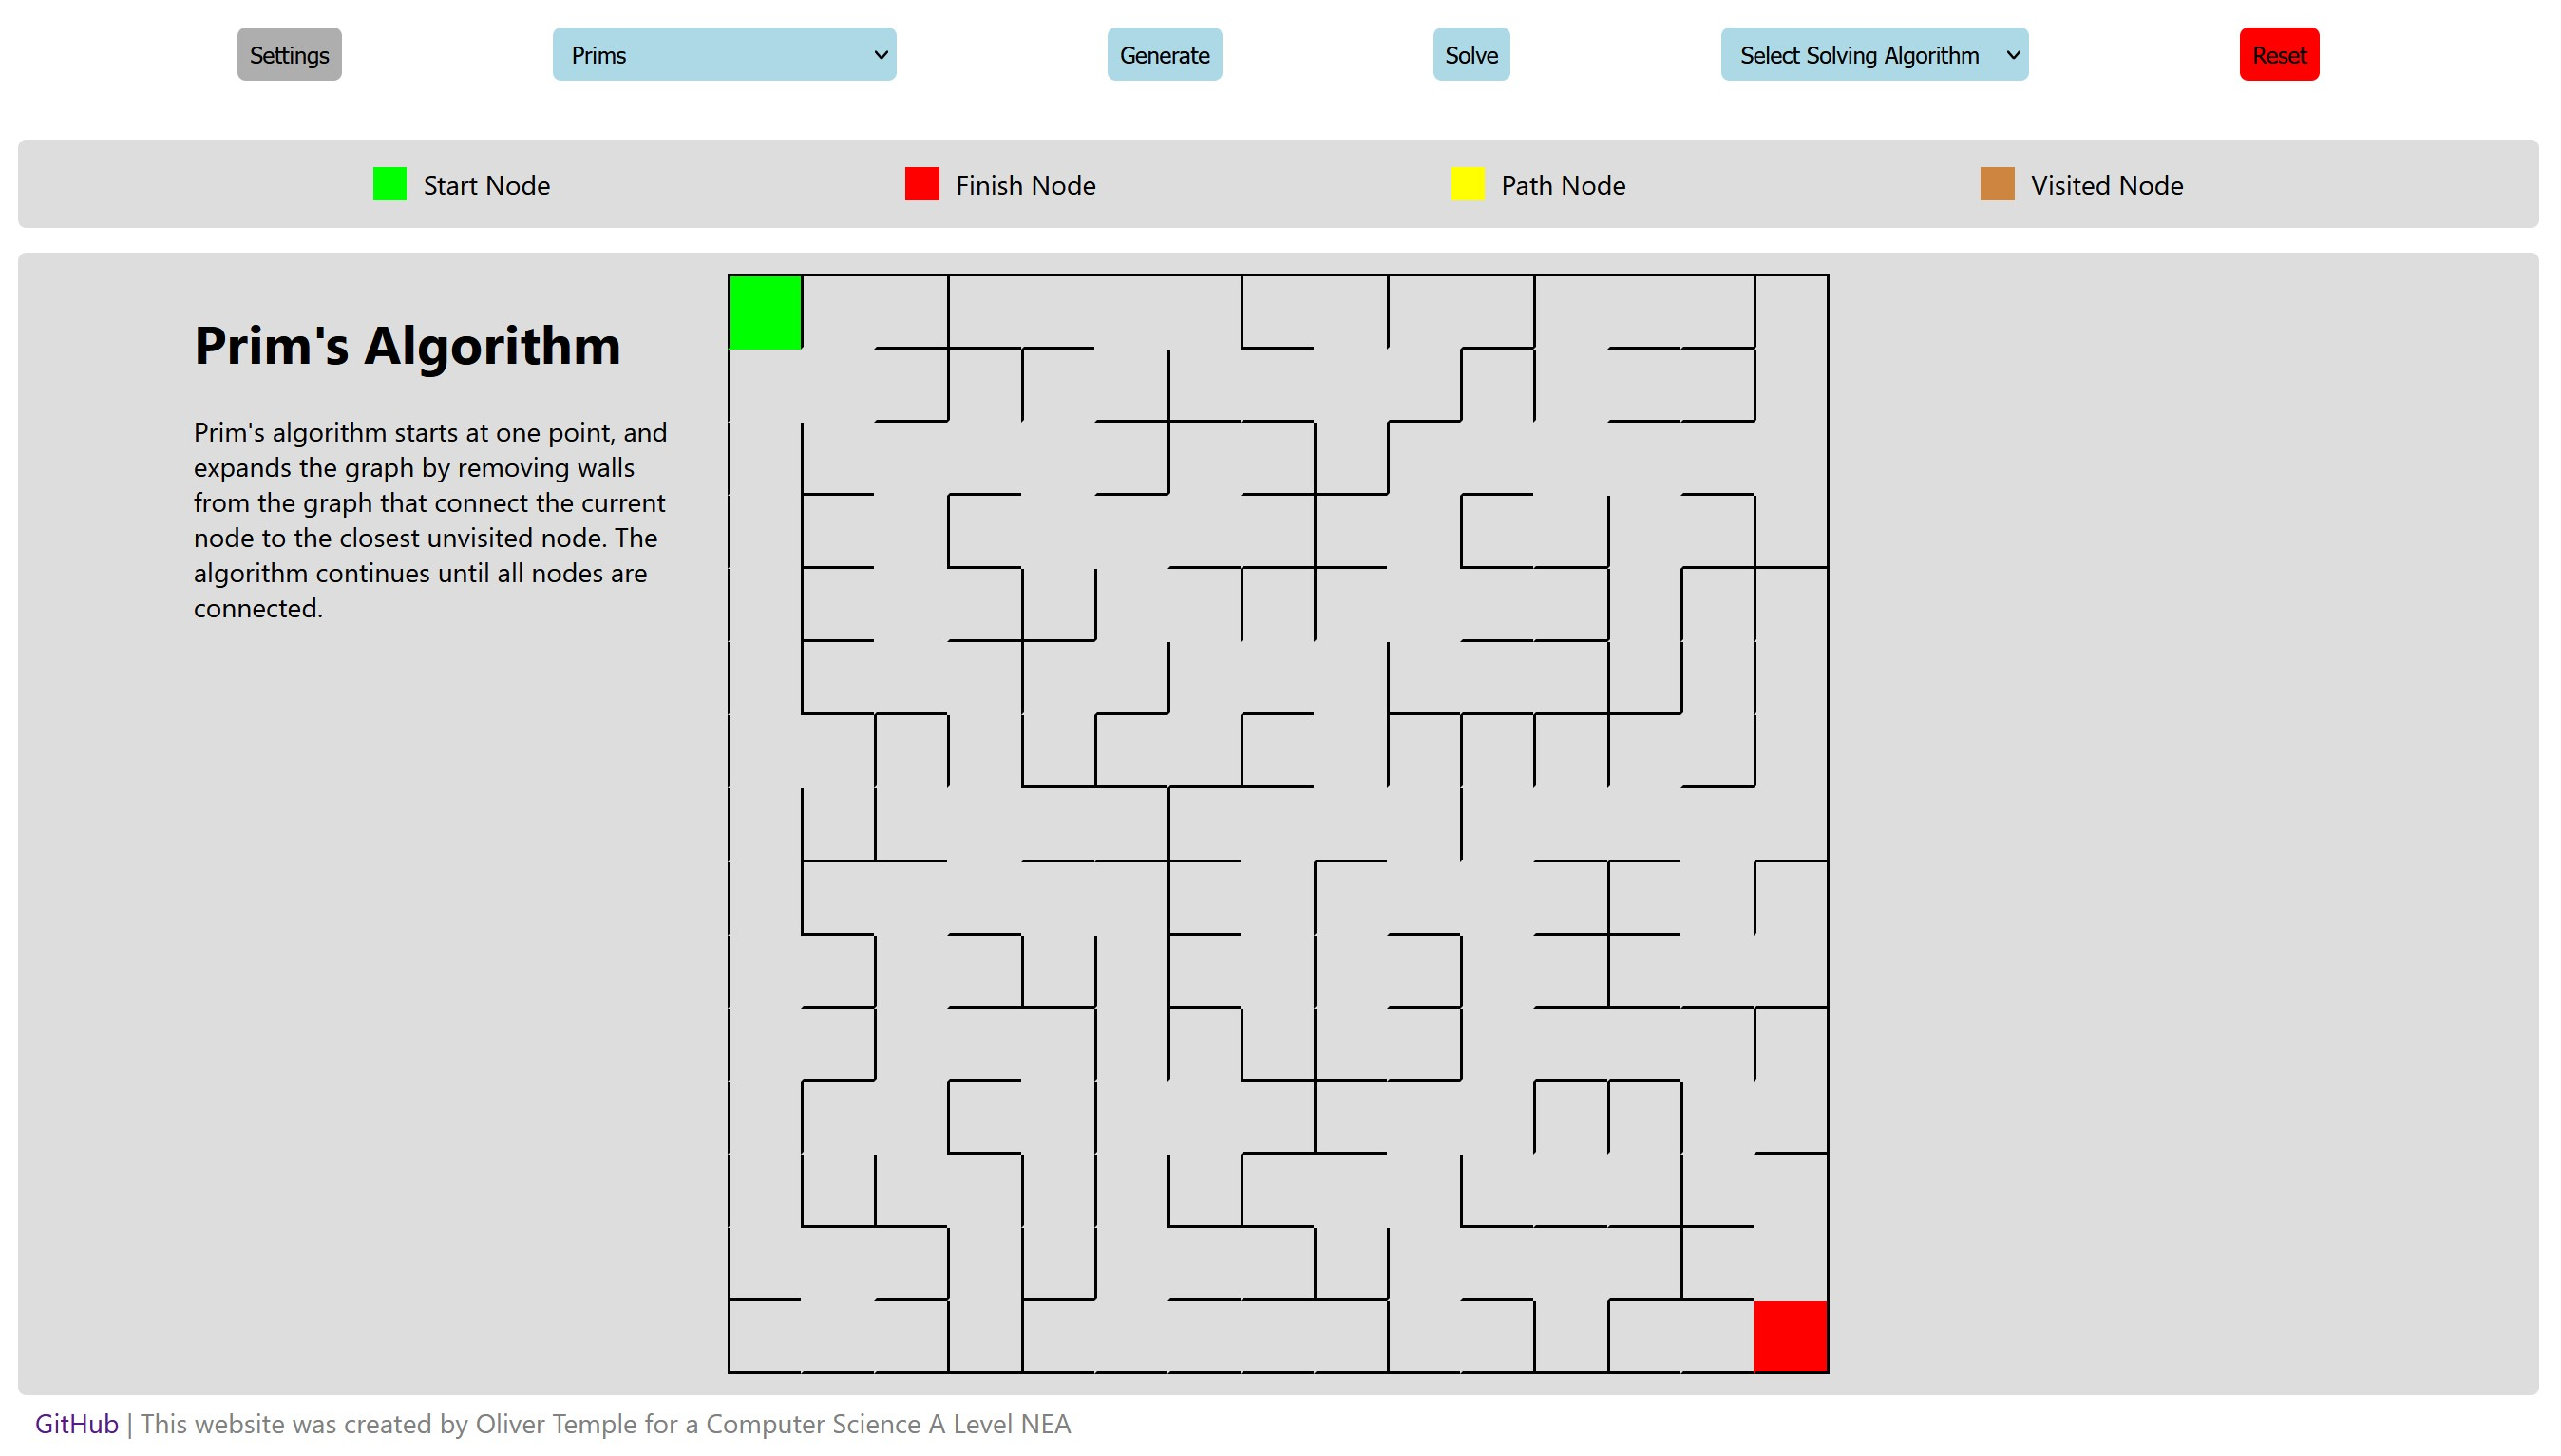
\includegraphics[width=\linewidth]{assets/testing/test3a.jpg}
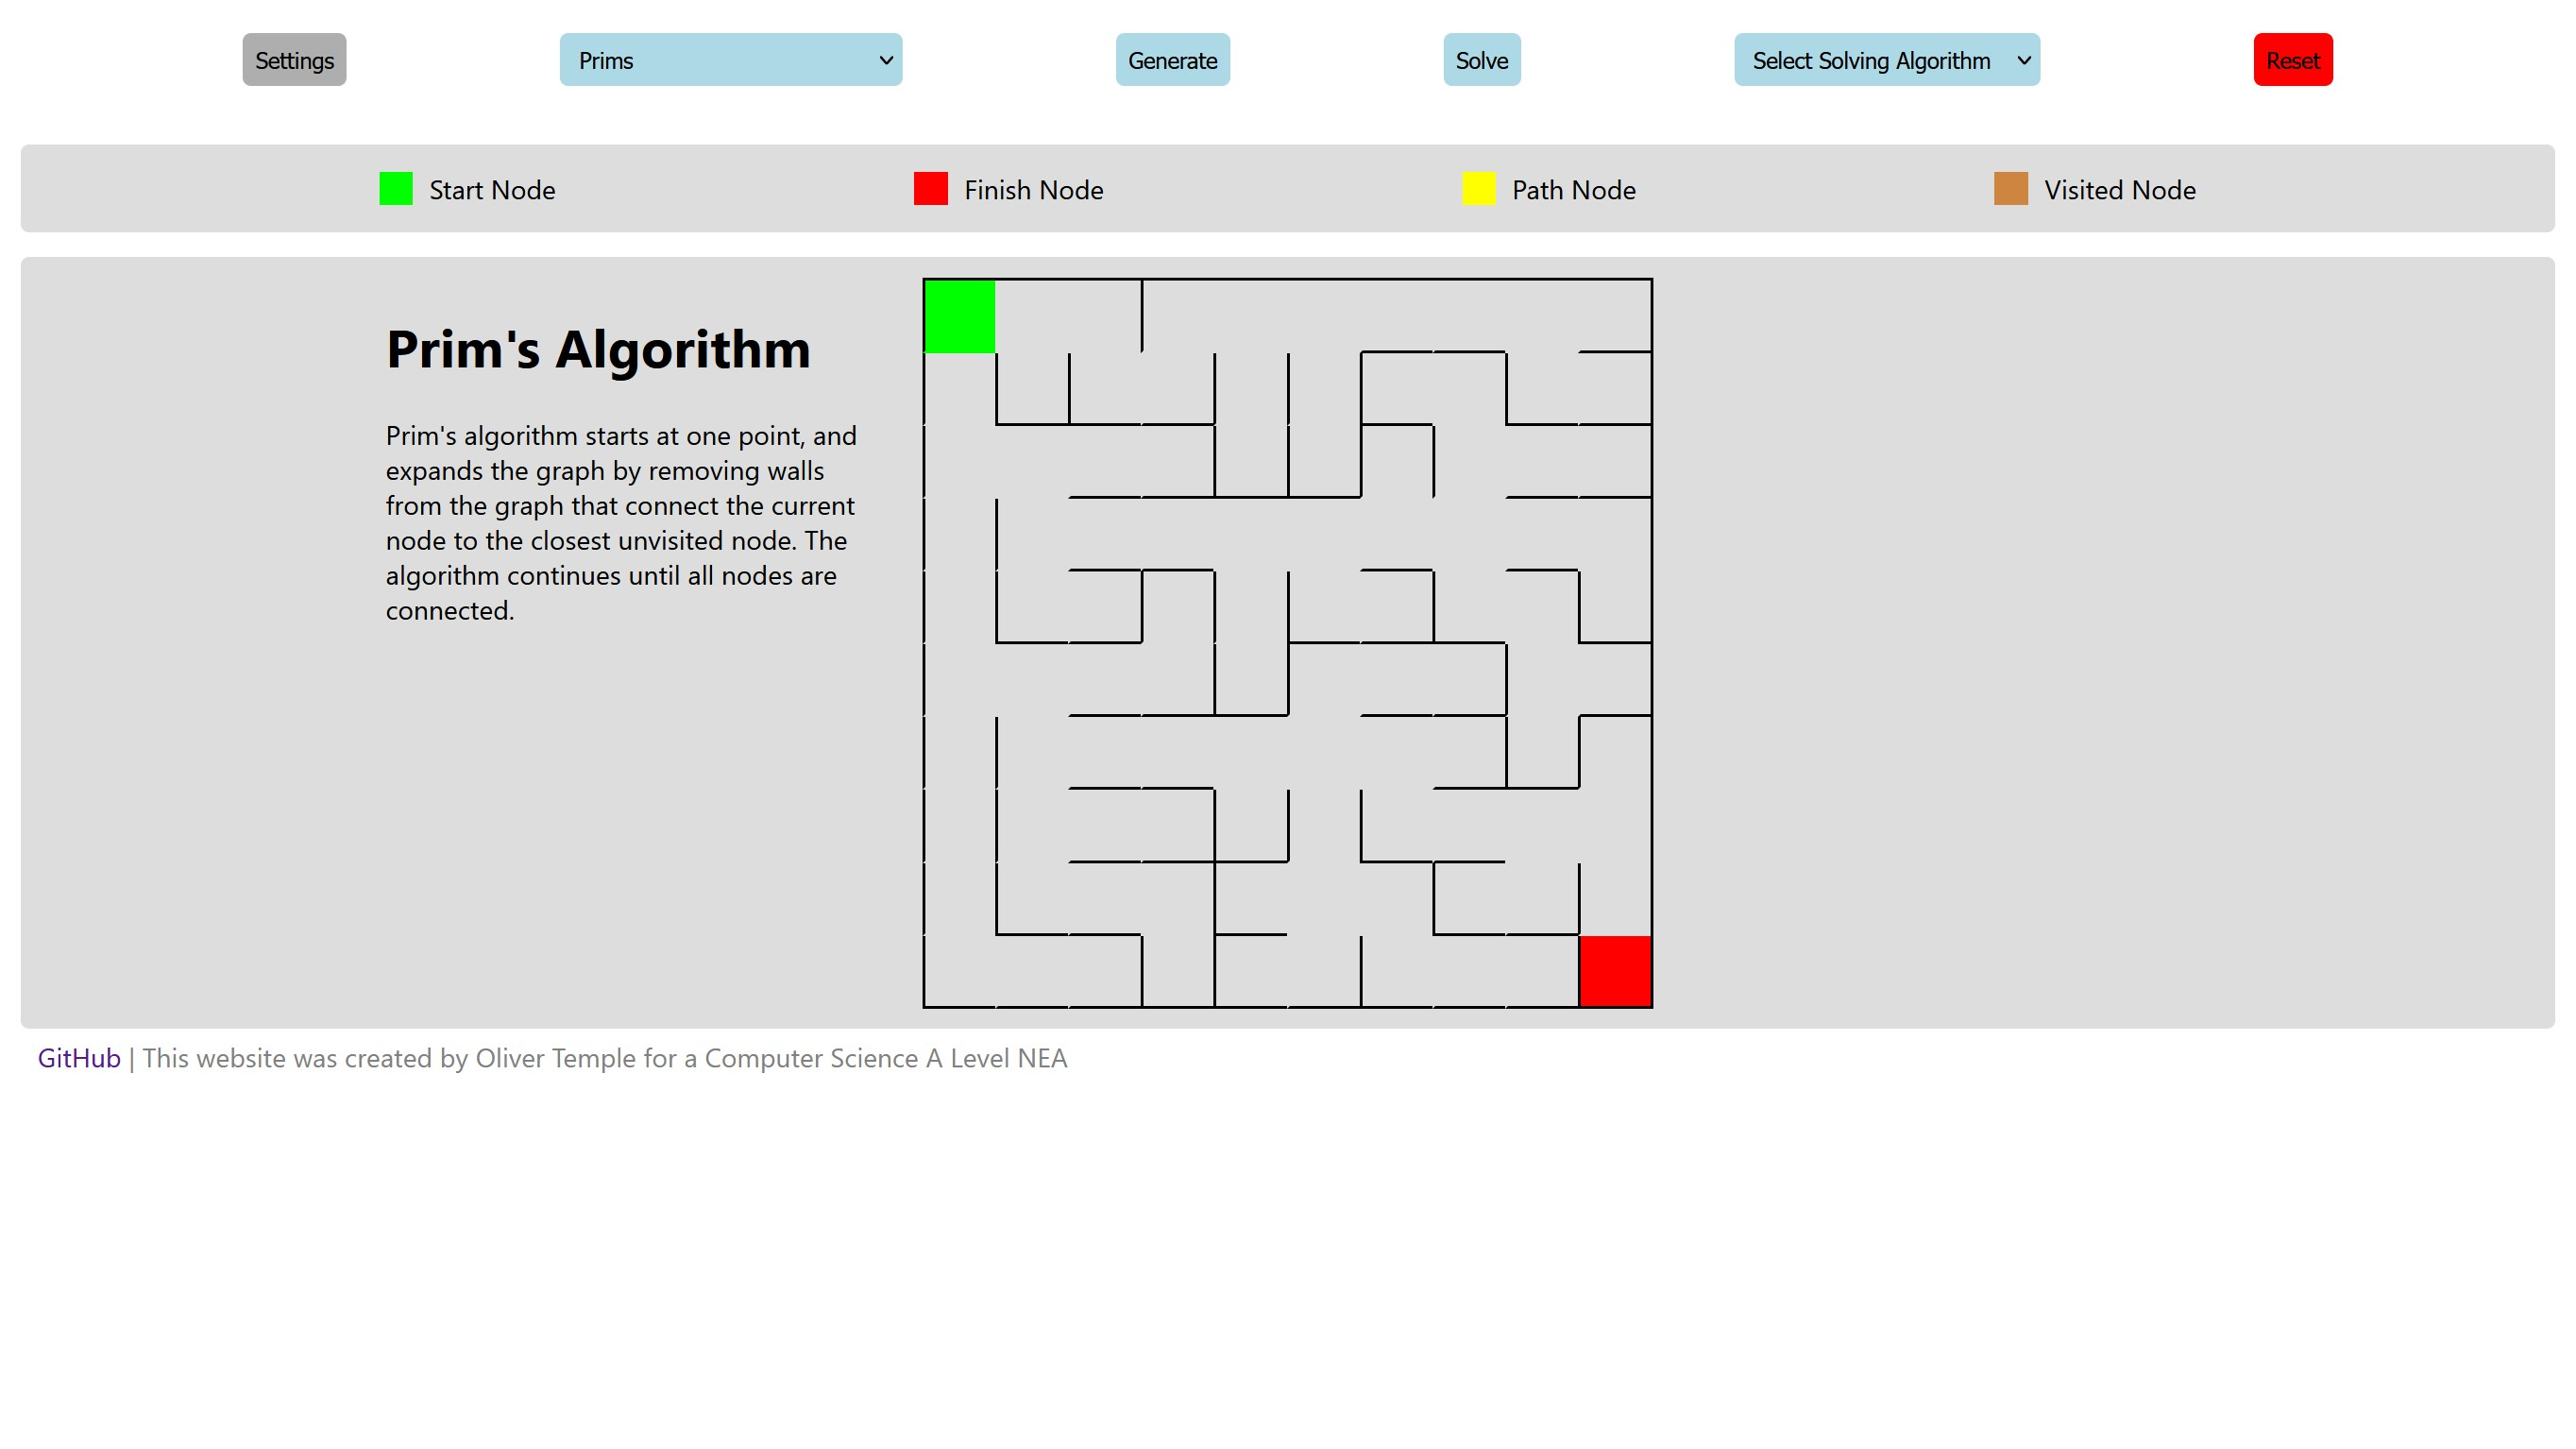
\includegraphics[width=\linewidth]{assets/testing/test3b.jpg}

\subsubsection{Recursive Backtracking}
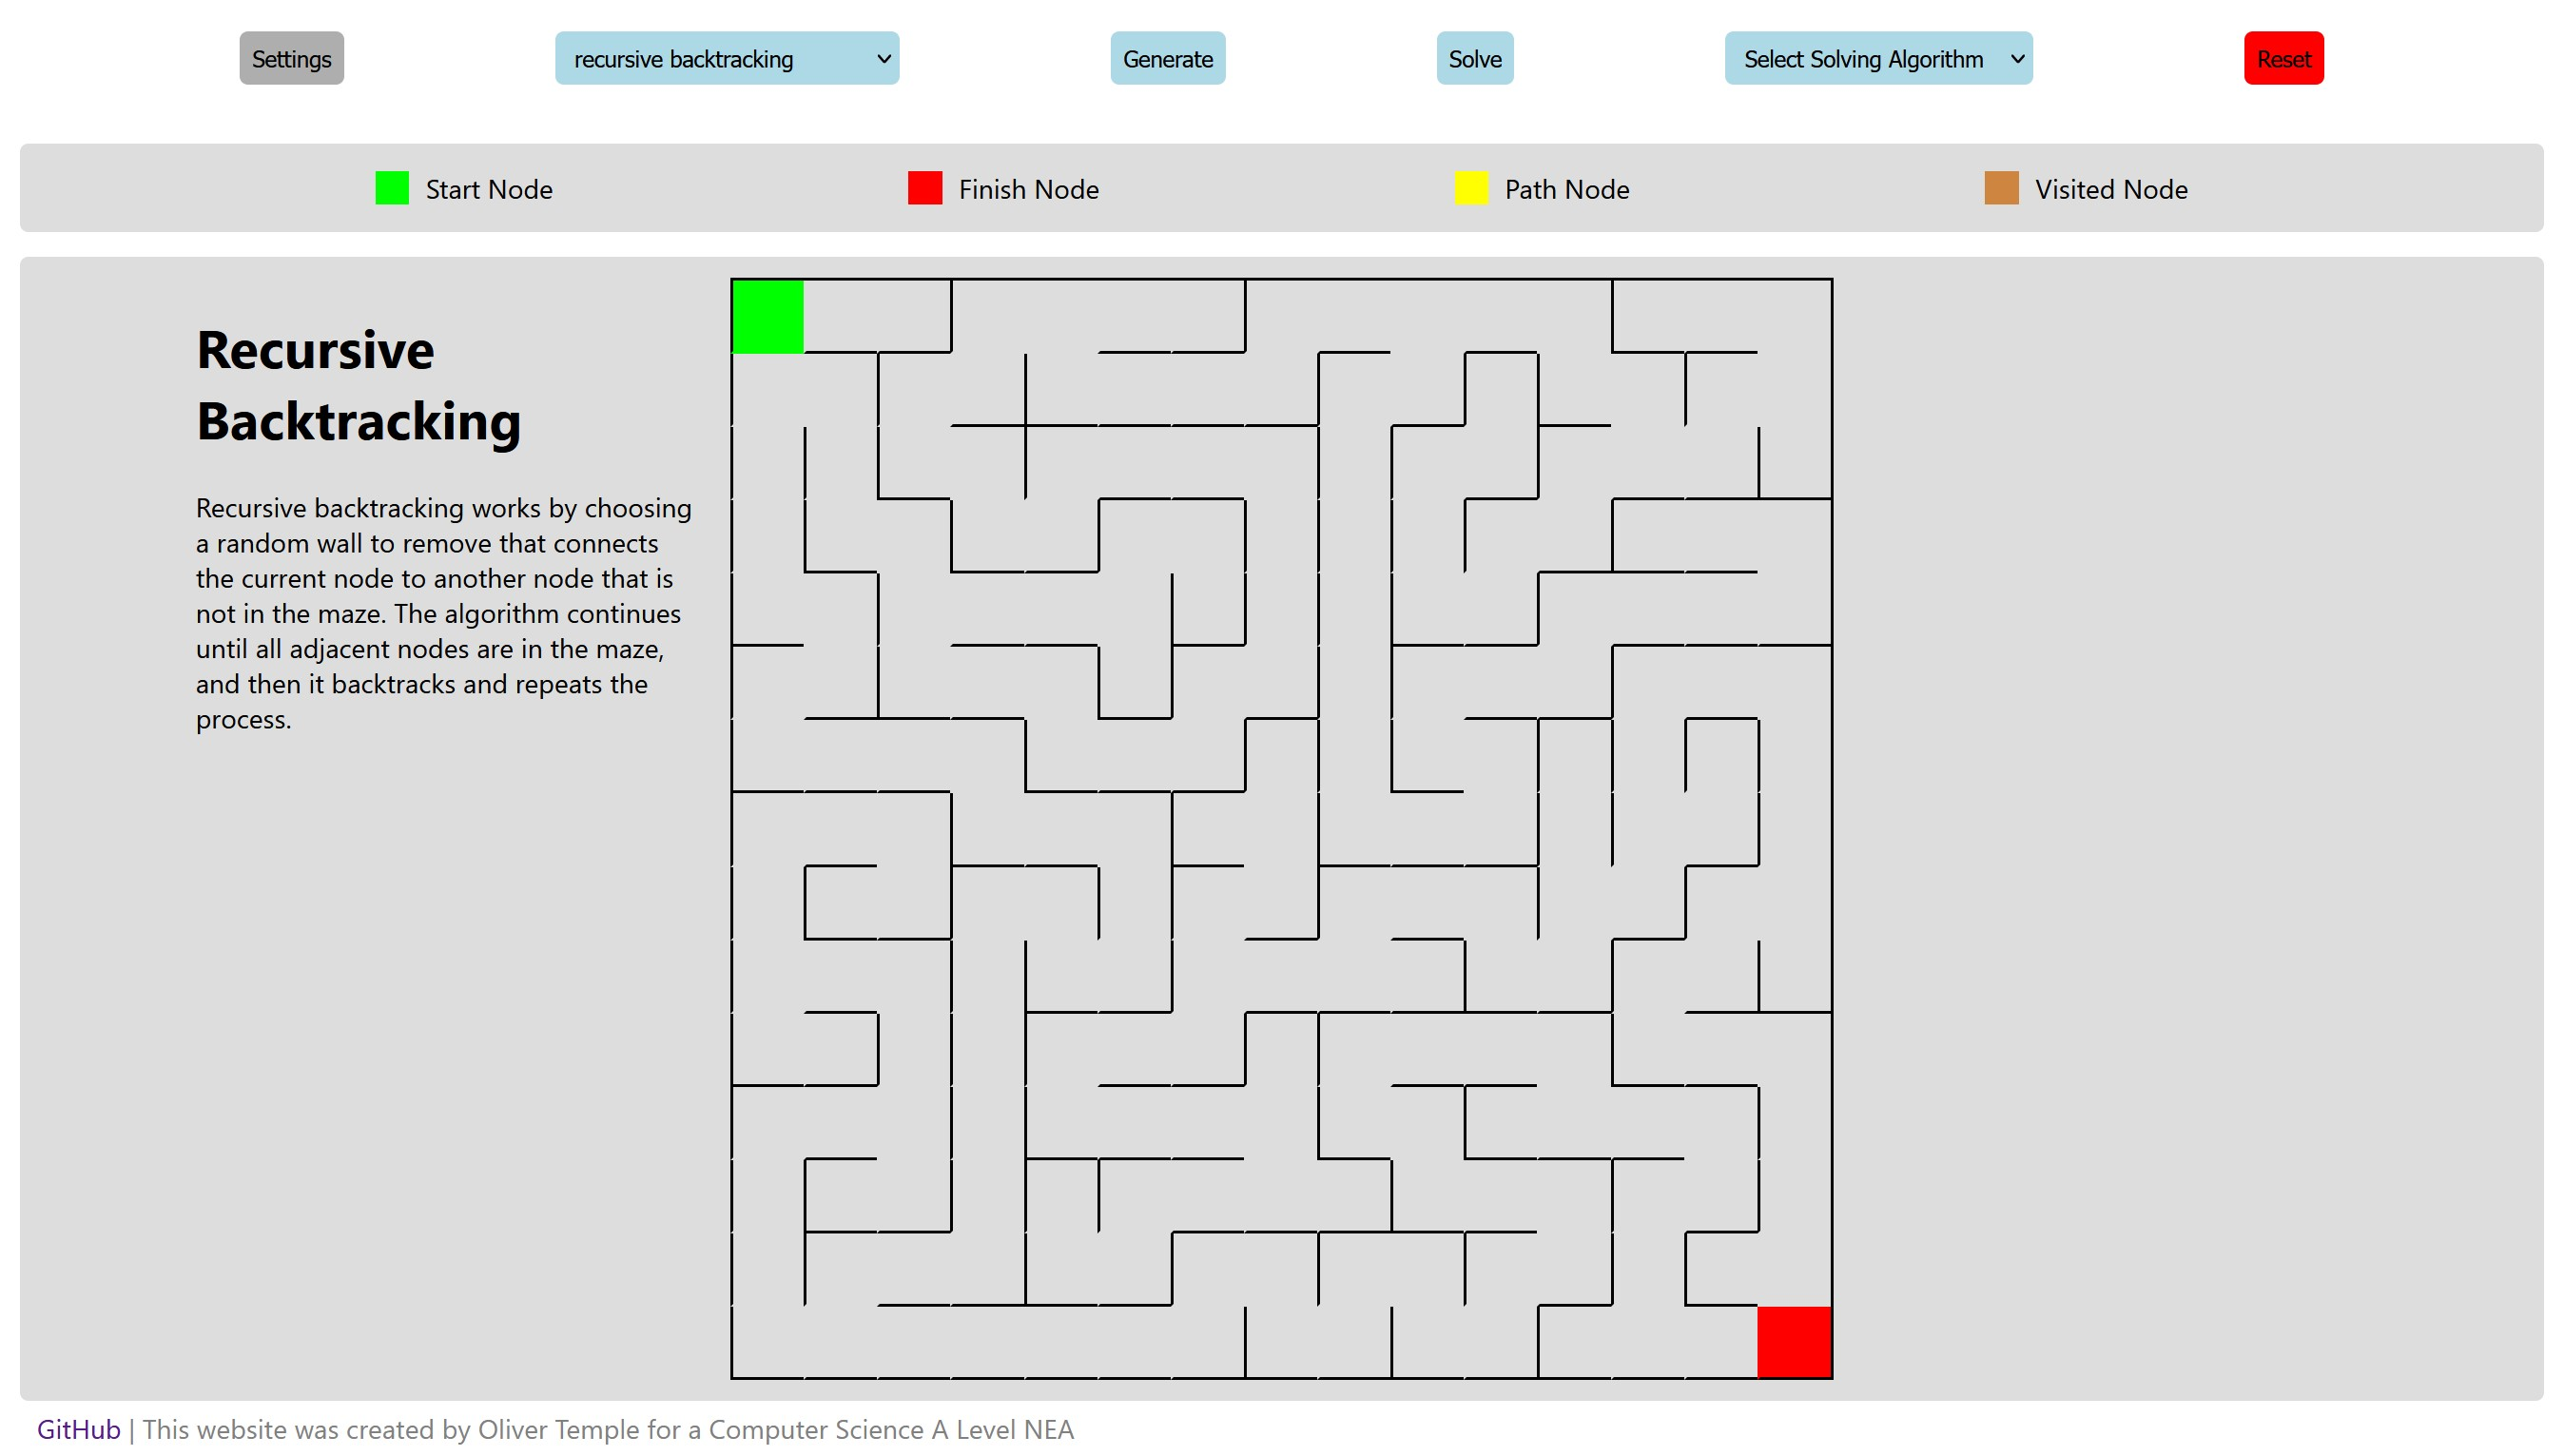
\includegraphics[width=\linewidth]{assets/testing/test3c.jpg}
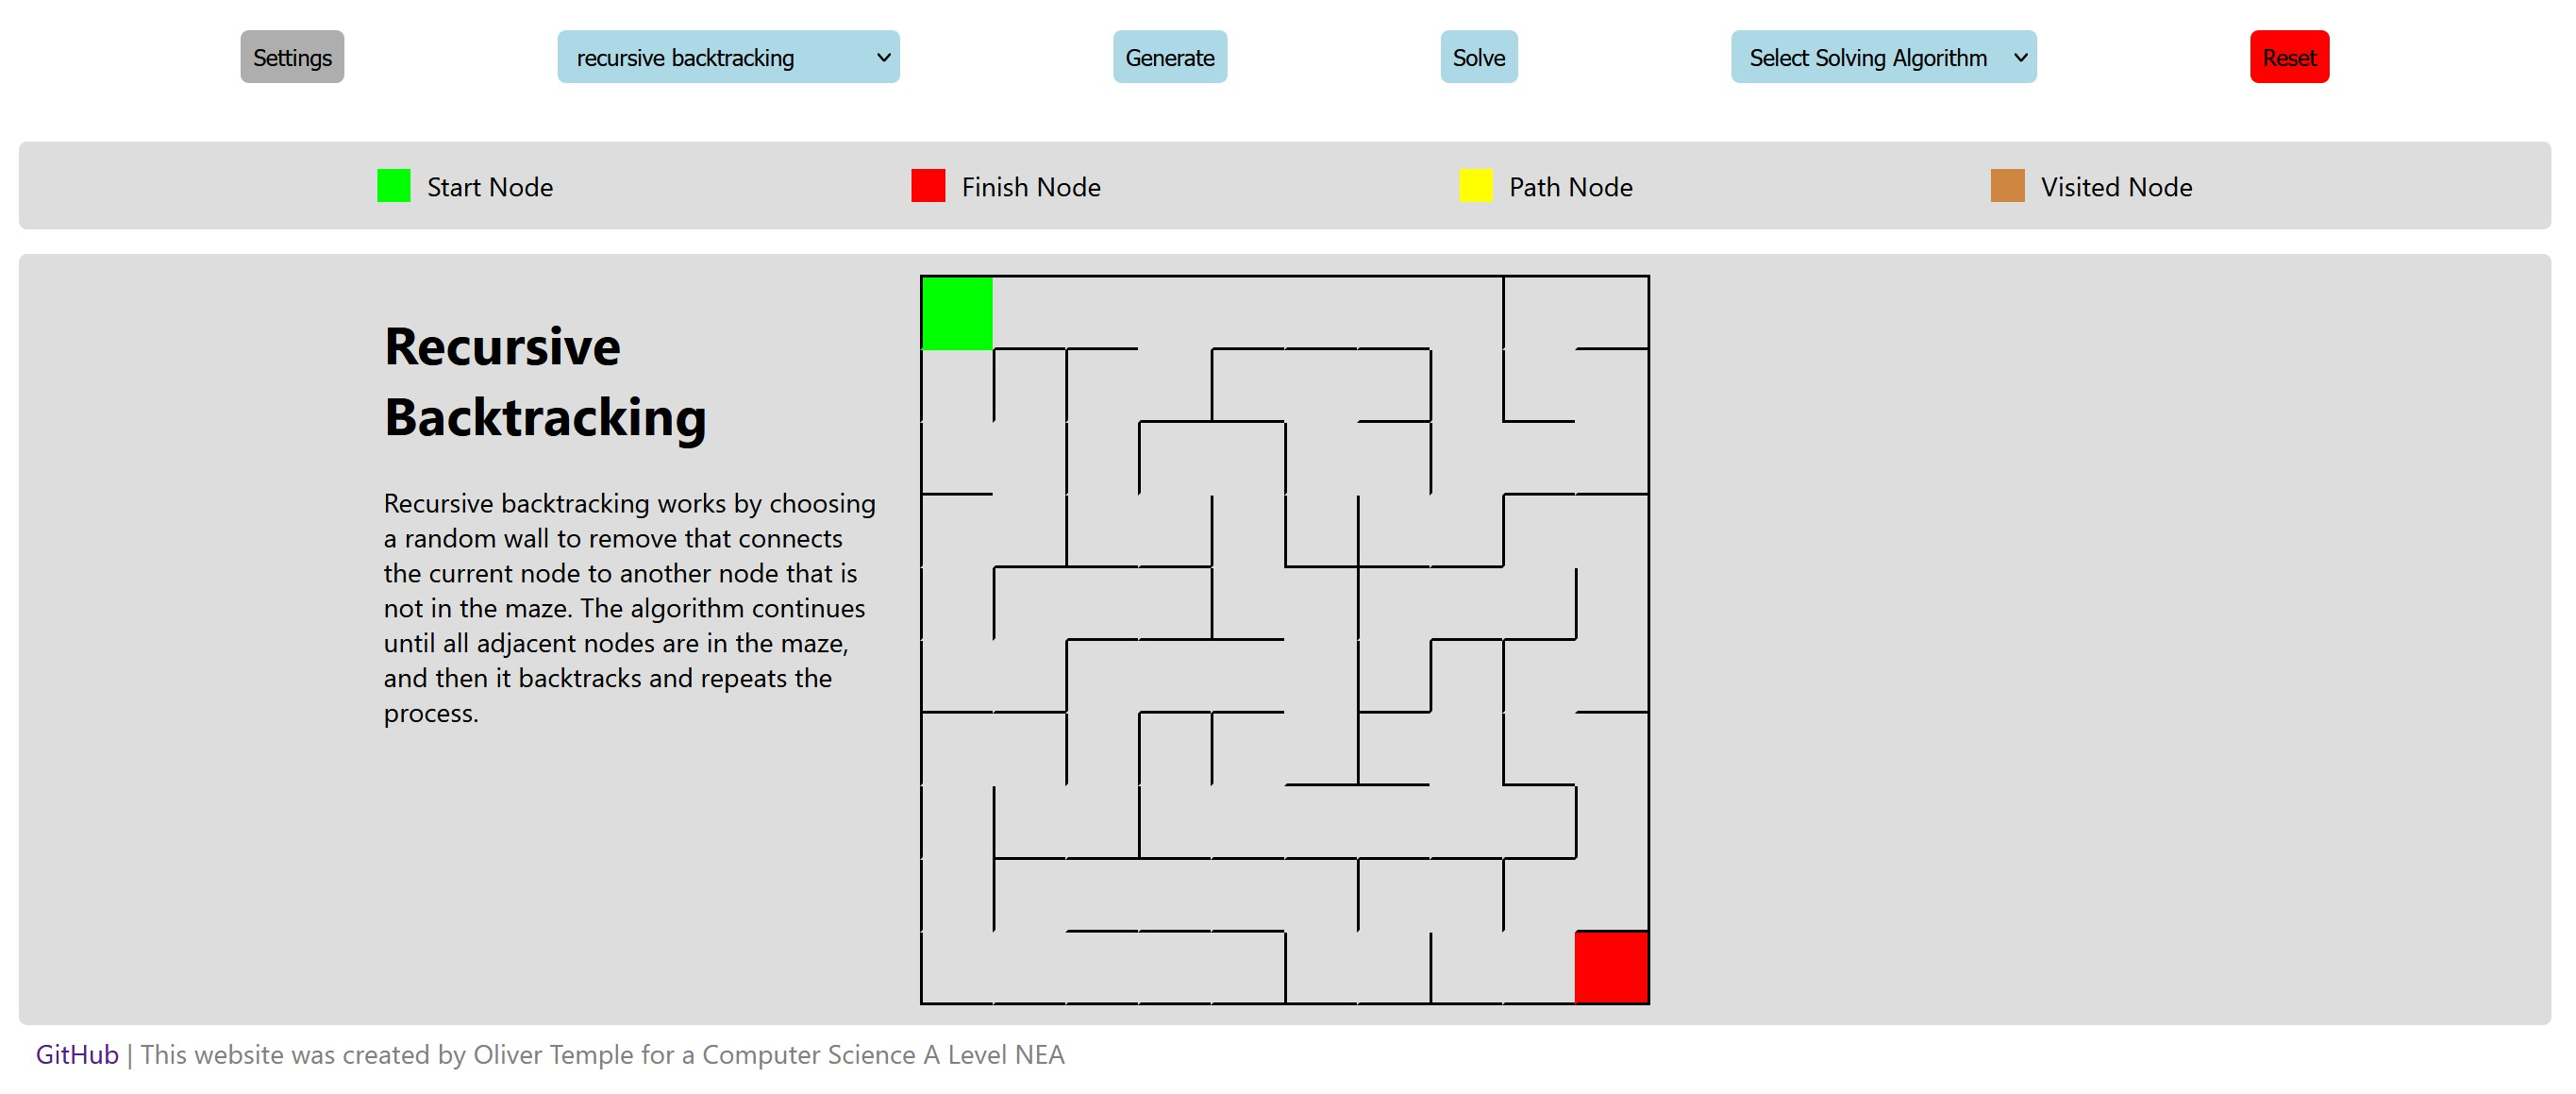
\includegraphics[width=\linewidth]{assets/testing/test3d.jpg}

\subsection{Test4/Test5: Pass}
Blow are links to videos assorted mazes being solved using each of the different algorithms, with different speeds and sizes.
\subsubsection{Dijkstra's Algorithm}
\url{https://youtu.be/91A-1P_atU8}
\subsubsection{Depth First Search}
\url{https://youtu.be/wustNAgCnUk}
\subsubsection{Breadth First Search}
\url{https://youtu.be/9y0Rl22FHVo}
\subsubsection{Greedy Search Manhattan}
\url{https://youtu.be/vOa5Yzk5X8c}
\subsubsection{Greedy Search Euclidean}
\url{https://youtu.be/PcCLCc52ujs}
\subsection{Test6: Pass}
When the reset button is pressed, an empty grid of the current size is generated. \url{https://youtu.be/kffa8GjnVL4}
\subsection{Test7}
When moving the start and finish nodes, the maze is resolved, however, sometimes the colours of the start or end nodes are not update properly when they are moved.
\url{https://youtu.be/0yQi2wyBA7Y}

\section{Evidence of Completeness}  
\subsection{Objectives Again}
\subsubsection{Generate Mazes}
The website should be able to generate mazes using multiple algorithms, including, but not limited to: Prim's algorithm and recursive backtracking. There should also be a brief description of the algorithm that has been selected.

\subsubsection{Solve Mazes}
The website should be able to solve mazes using multiple algorithms, including, but not limited to: greedy search, Dijkstra's algorithms, depth-first search and breadth-first search. There should also be a brief description of the algorithm that has been selected.

\subsubsection{Customisation}
The user should be able to customize aspects of the visualization, including:
\begin{itemize}
    \item Size of the maze.
    \item Speed of the animation.
    \item The heuristic used in any heuristic algorithms.
\end{itemize}

\subsubsection{User written algorithms}
The website should be able to run algorithms written by the user for both maze generation and solving. This will be done by supplying documentation on what parameters need to be taken in and what will need to be returned from the function for the visualizer to work.

\subsubsection{Update Visualization}
If the start or end nodes are moved once the visualization has been run, then it should update without the user having to rerun the visualization.

\subsection{Analysis of Objectives}
\subsubsection{Generate Mazes}
The project is able to generate mazes using multiple algorithms, as stated in the objective above. The available algorithms for generating mazes are:
\begin{itemize}
    \item Prim's Algorithm
    \item Recursive Backtracking
\end{itemize}
These were the algorithms that were asked for by the prospective user, and that were in the objective above, as well as give a brief description of each algorithm. Unfortunately, I was unable to implement Kruskal's algorithm, as I did not have time, however, this was less important to the end user, so I feel that this does not effect the completeness of the project.

\subsubsection{Solve Mazes}
The project is able to solve mazes using multiple algorithms, as stated in the objective above, as well as give a brief description of each algorithm. The available algorithms for solving mazes are:
\begin{itemize}
    \item Dijkstra's Algorithm
    \item Depth First Search
    \item Breadth First Search
    \item Greedy Search (Manhattan)
    \item Greedy Search (Euclidean)
\end{itemize}
These were the algorithms that were stated in the objective above, and include the request from the objective user, that there should be an algorithm as well as a heuristic. I feel that the breadth first search and depth first search make a good addition to the project, as they are algorithms that are studied in A Level Computer Science, and one of the purposes of this project is for it to be used in classrooms.

\subsubsection{Customisation}
All of the options for customization in the objective has been implemented into the project. The user can change the size of the maze, the speed of the animation, and the heuristic used in the greedy search algorithms.

\subsubsection{User written algorithms}
Unfortunately, the project is unable to run user written algorithms. This is because I have implemented a client server model, where the algorithms are run on the API, and it would be unsafe to run user written code on the API without first parsing and sanitizing the code, which is beyond the scope of this project.

\subsubsection{Update Visualization}
The project is able to update the visualization without the user having to rerun the visualization when the start or end nodes are moved, as stated in the objective above.

\section{Evaluation}
\subsection{Independent Feedback}
I wanted to go back to the end users with the finished visualization, to see if they had any feedback on the project or any ideas on further improvements that could be made.
There feedback was:
\begin{itemize}
    \item[Item 1.]"The user interface was intuitive on the whole, however, I feel that the solve button should be on the other side of the solving algorithms dropdown."
    \item[Item 2.]"I thought that the menus were intuitive, and that the key was very useful to know what the different coloured squares meant."
    \item[Item 3.]"I thought that the information on the algorithms was of a good length."
    \item[Item 4.]"If a size rather higher than 30 is entered, no message is shown as to why a new maze is not being generated."
    \item[Item 5.]"I think it would be nice if I could download a gif of the maze being solved."    
    \item[Item 6.]"I think that the visualization was high tier."
    \item[Item 7.]"It would be nice if there were more maze generating algorithms, such as Kruskal's algorithm."  
\end{itemize}
\subsection{Response to Independent Feedback}
\subsubsection{User Interface}
In response to item 1, I have moved the solve button to the right of the solving algorithms dropdown, as shown in the image below.
\newline
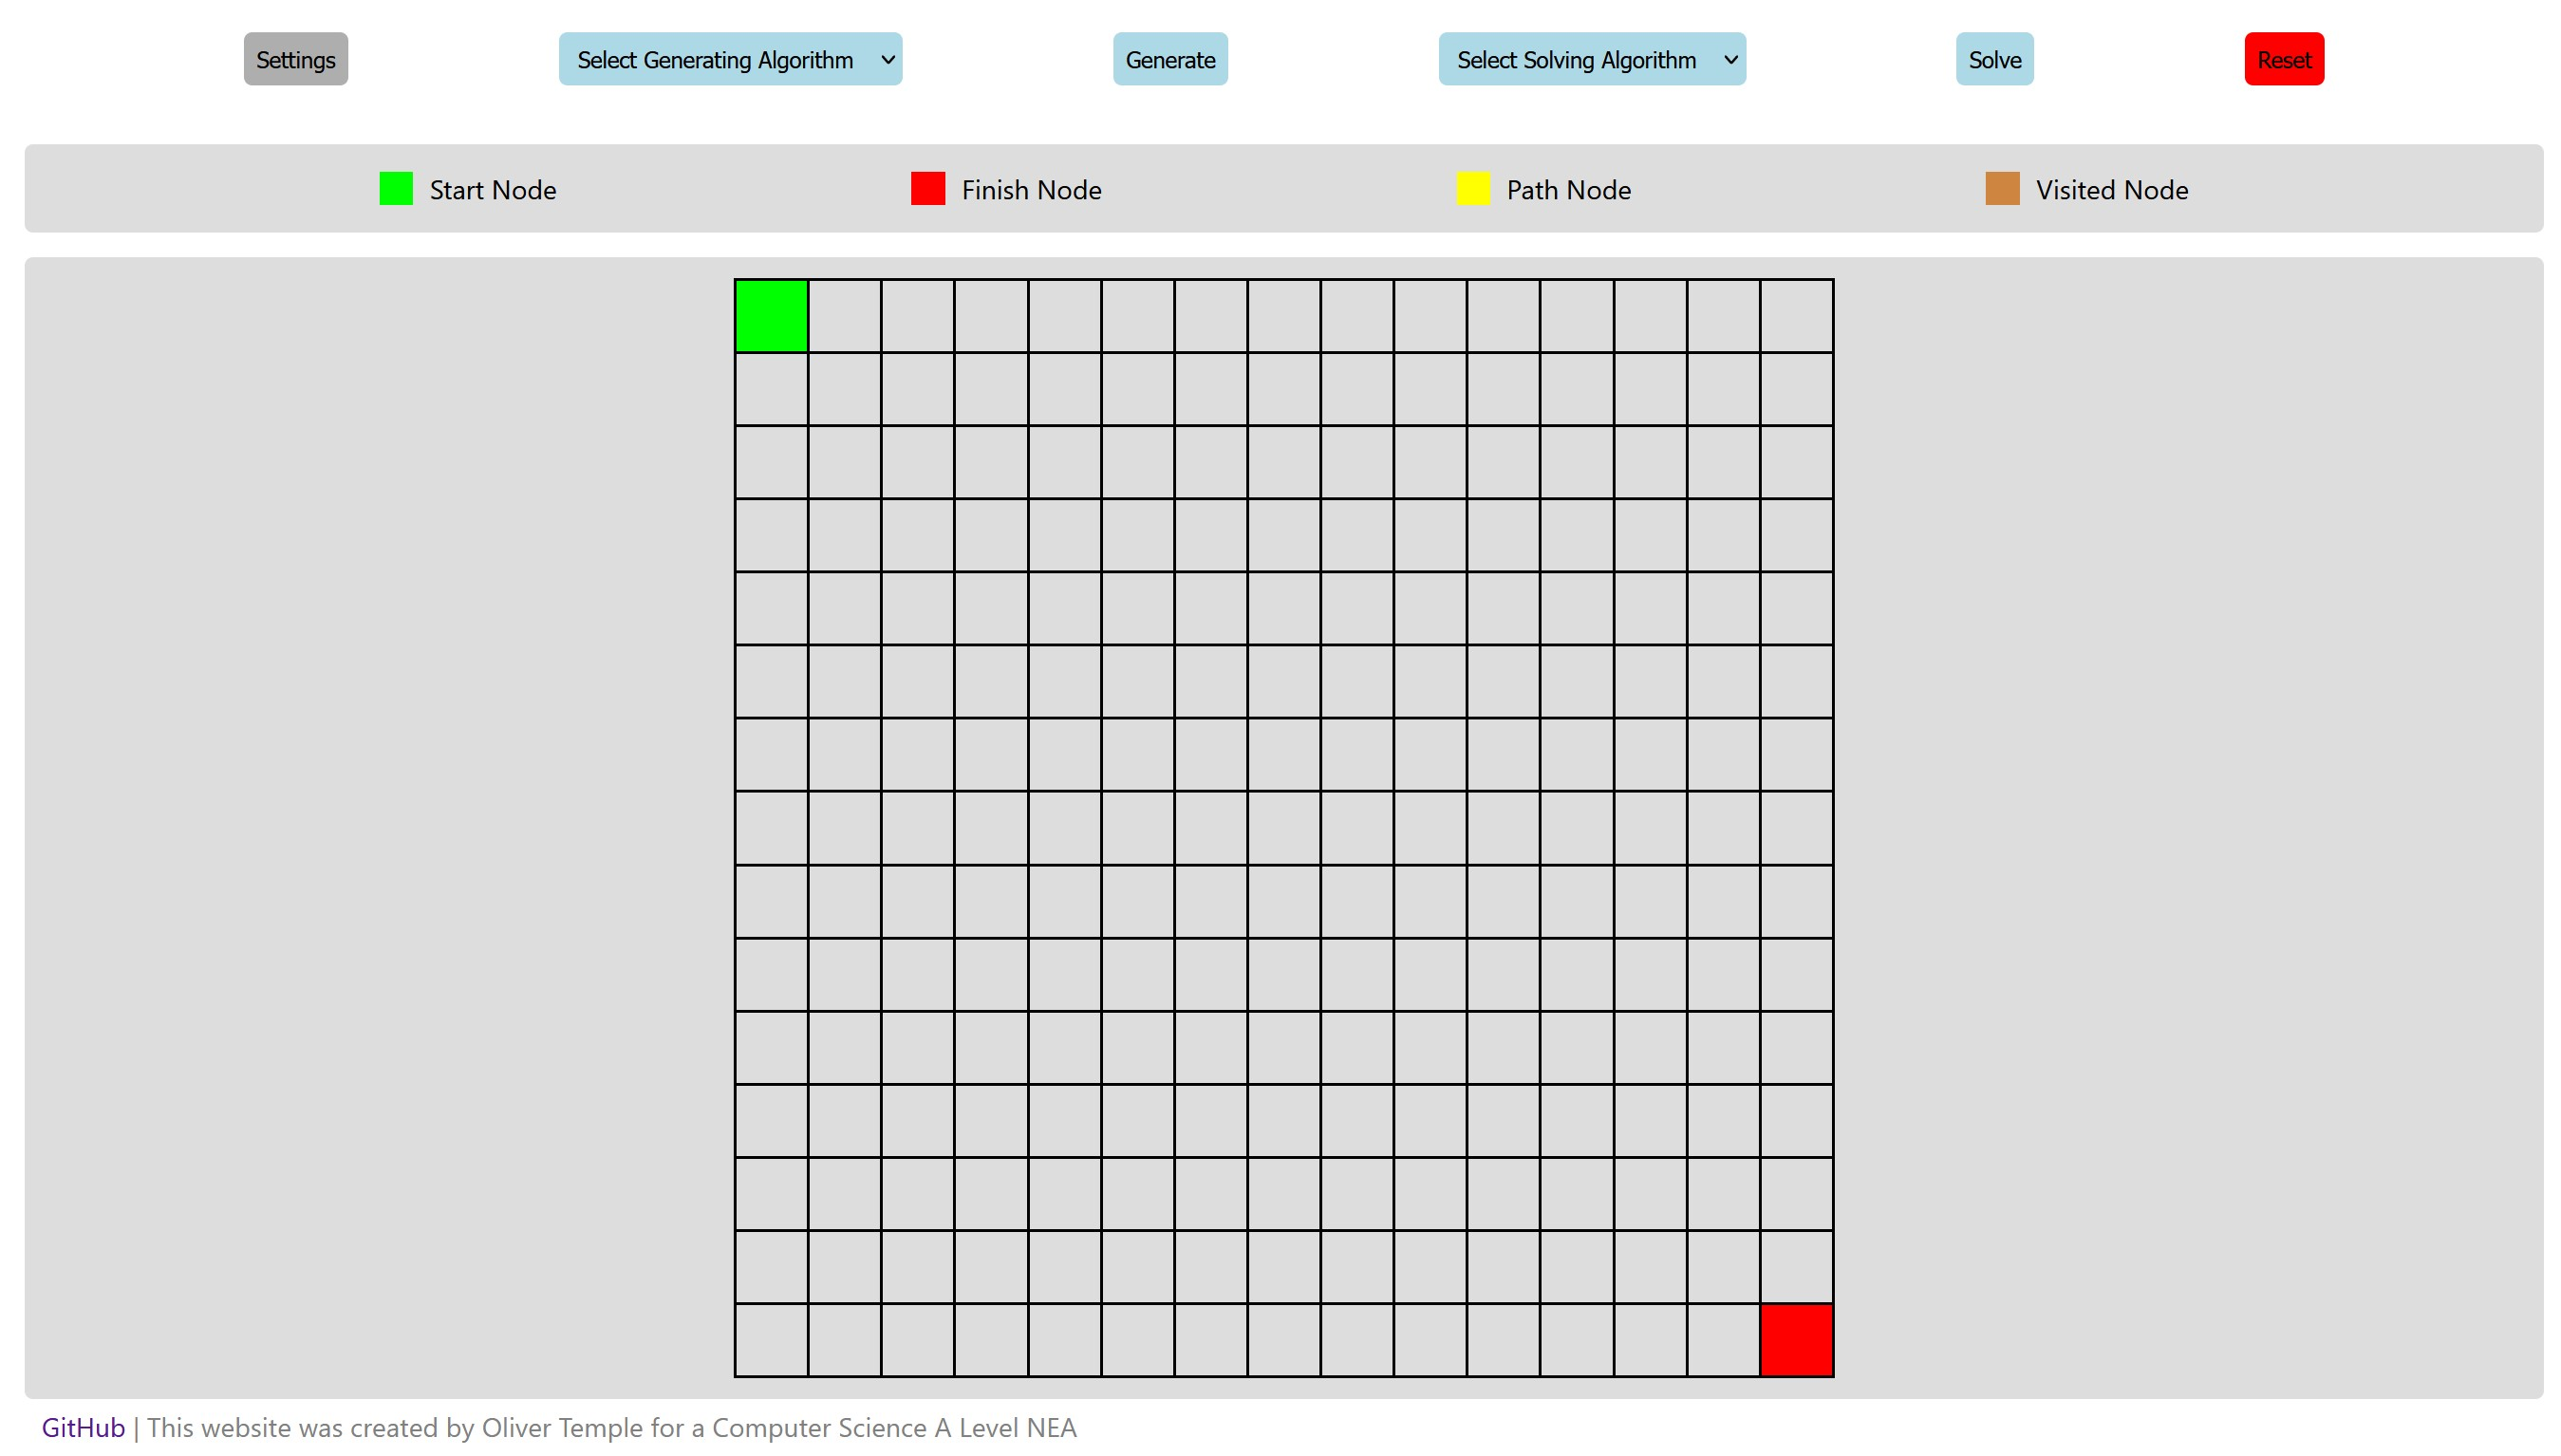
\includegraphics[width=\linewidth]{assets/feedback/item1.jpg}

\subsubsection{Max Size Error}
In response to item 4, I have added an alert if a size above 30 is entered, which will tell the user why a new maze is not being generated, as shown in the image below.
\newline
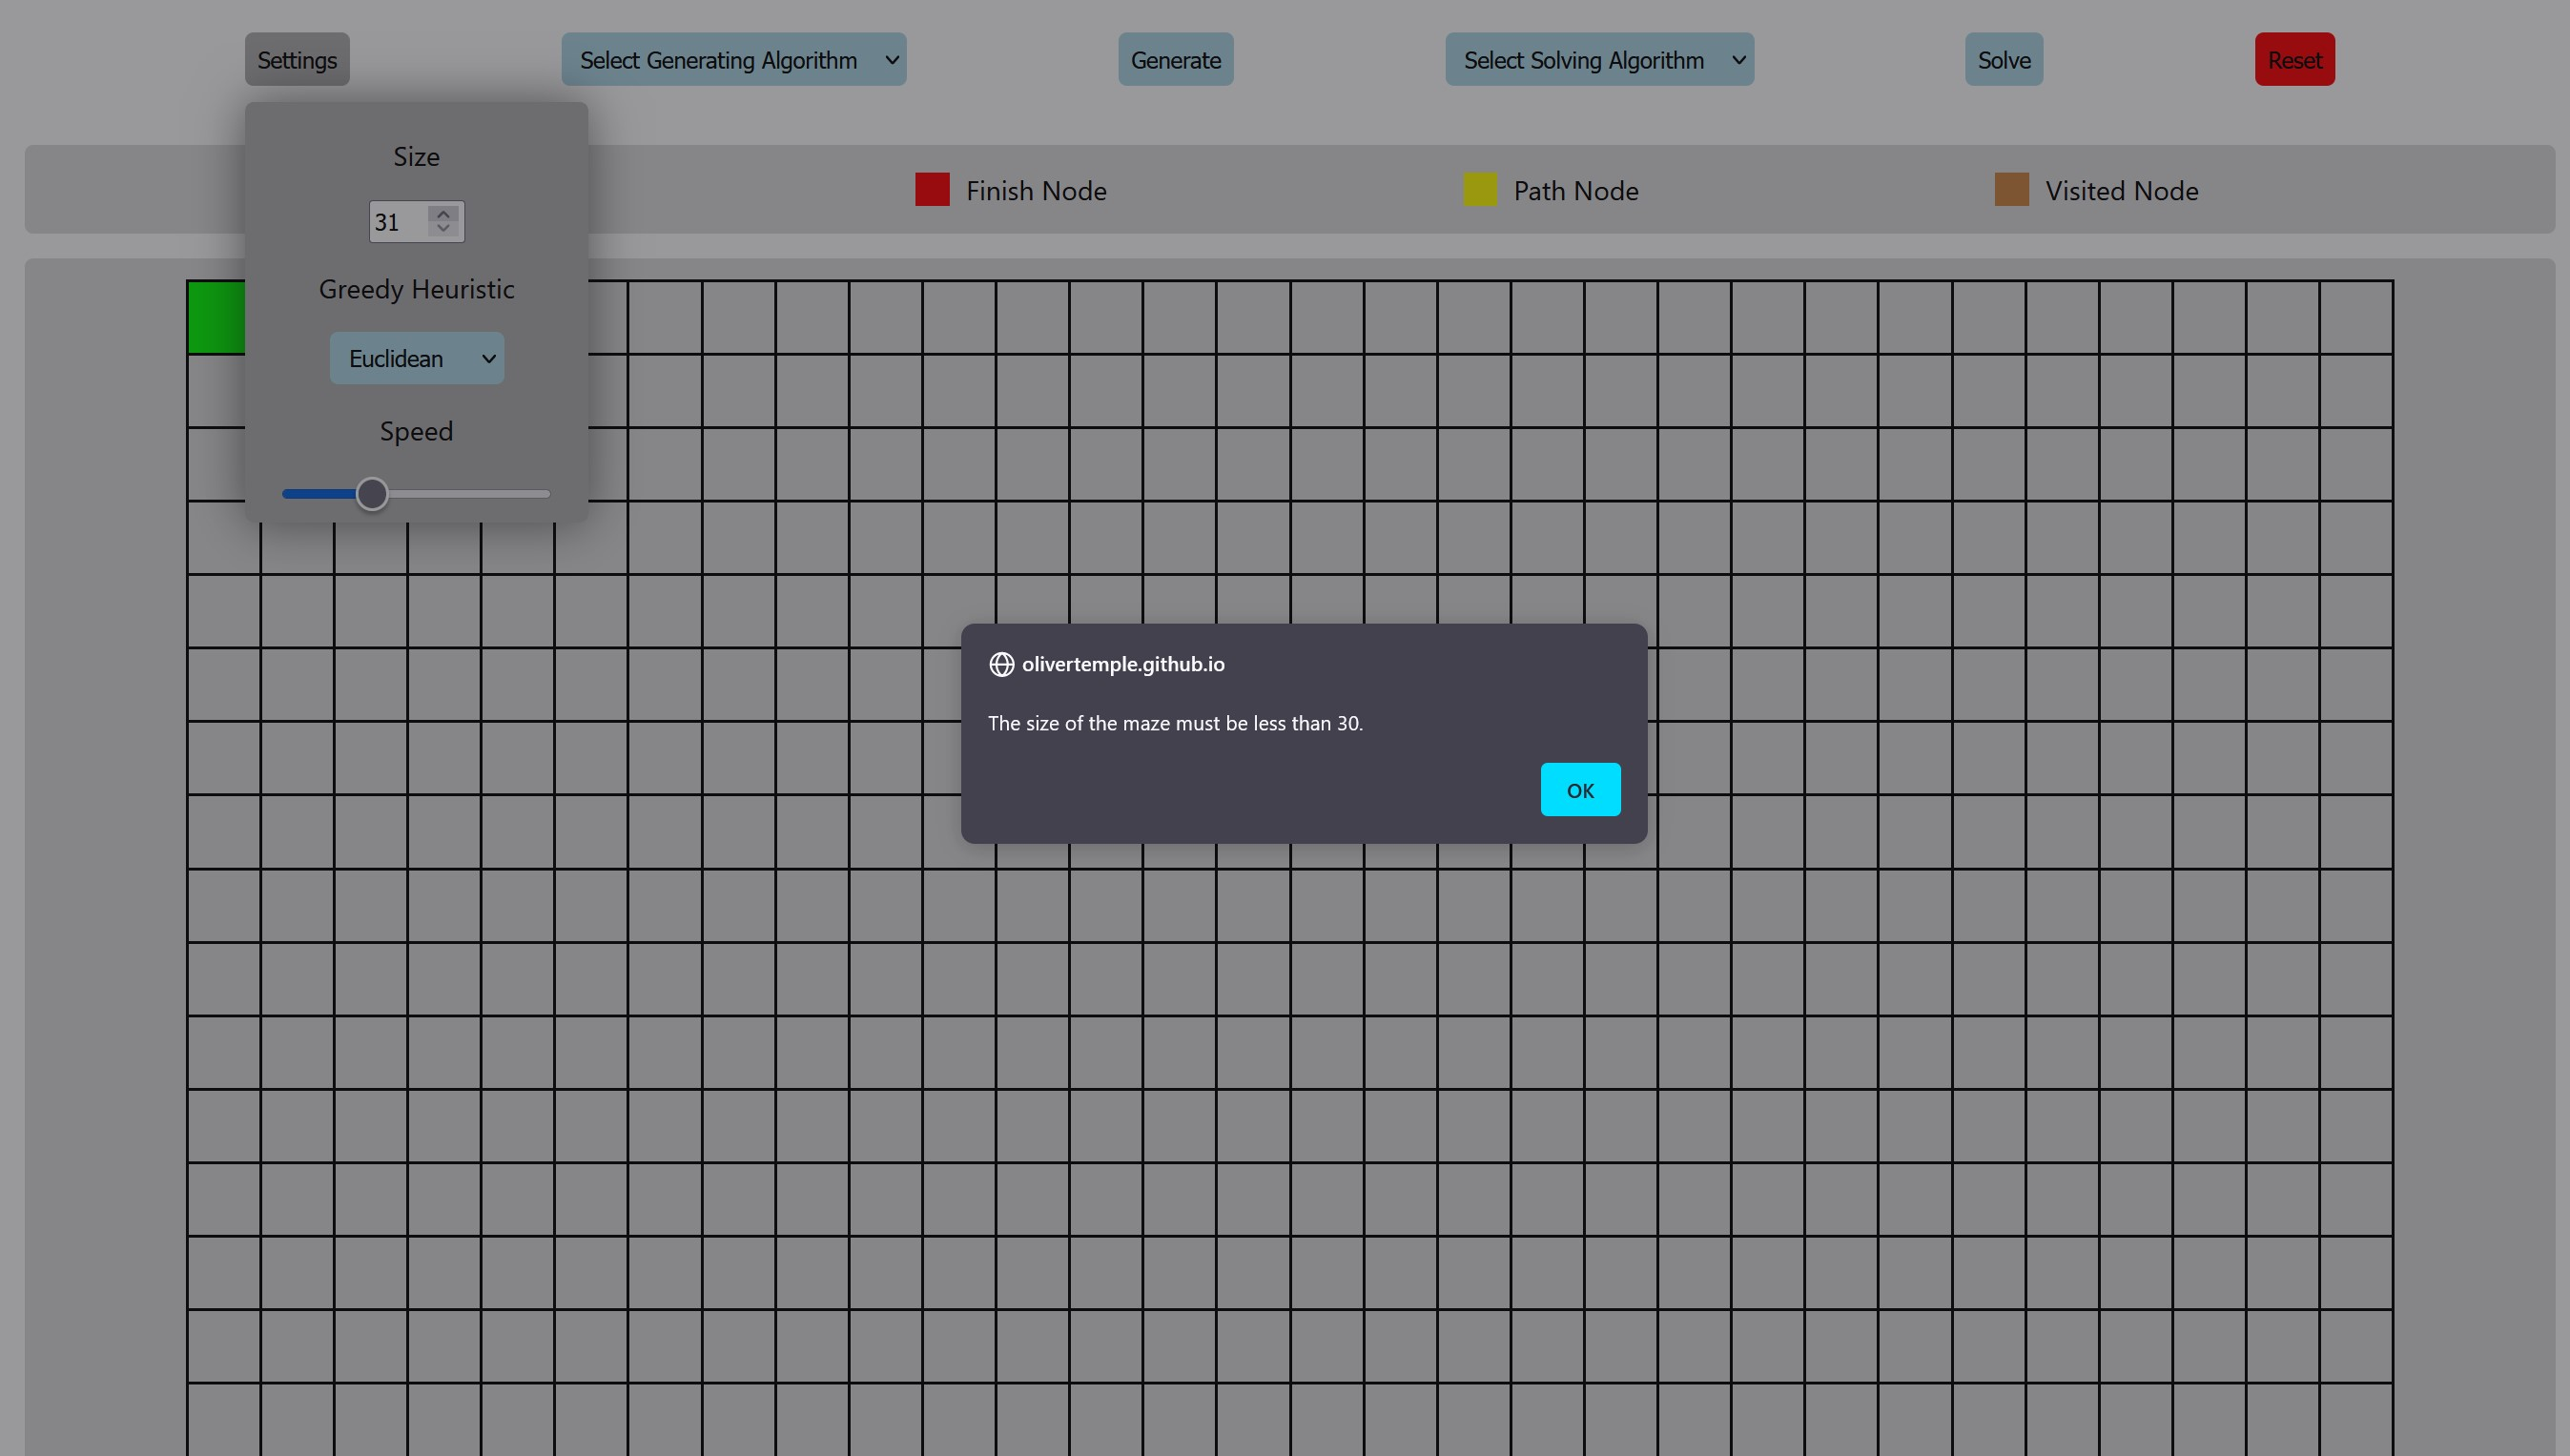
\includegraphics[width=\linewidth]{assets/feedback/item4.jpg}

\subsubsection{Gif}
Although I think that being able to download a gif of the maze being solved would be a beneficial feature, it would require a lot of work on the back end, as there is no software for visualizing the maze being solved in the api. Because of this, I have put it into the "Improvements that could be made" section.

\subsection{Improvements that could be made}
There a few improvements that I would make to this project if I had more time:
\begin{enumerate}
    \item Add a "via point" node that the user can drag and drop that the path must go through.
    \item Make the size of the maze squares automatically scale with the size of the maze, so that the user does not need to zoom out for larger mazes.
    \item Allow for rectangular mazes.
    \item User drawn mazes.
    \item Allow the user to download a gif of the maze being solved.
\end{enumerate}

\subsection{Evaluation}
I feel that this project has been a success, as almost all of the objectives have been completed. The only objective that was not completed was the user written algorithms, however, this was not completed due to the security risks of running user written code on the API.
\end{document}